			\documentclass [12pt]{article} \usepackage{multicol}
		\usepackage{array} \usepackage{geometry}
		\usepackage{graphicx} \graphicspath{
		{/Users/alirezafaridamin/Desktop/temp/images} }
		\usepackage[export]{adjustbox} \usepackage{placeins}
		\usepackage{amsmath}
		
		\usepackage{titlesec}
		\setcounter{secnumdepth}{4}
		
		\usepackage{hyperref}
		\begin{document}
		 \hypersetup{
    colorlinks,
    citecolor=black,
    filecolor=black,
    linkcolor=black,
    urlcolor=black }

         
			\hyphenchar\font=-1 \pagestyle{headings}
		\pagenumbering{arabic} \setcounter{page}{1}

	\let\Oldsection\section
\renewcommand{\section}{\FloatBarrier\Oldsection}

	\let\Oldsubsection\subsection
\renewcommand{\subsection}{\FloatBarrier\Oldsubsection}

	\let\Oldsubsubsection\subsubsection
\renewcommand{\subsubsection}{\FloatBarrier\Oldsubsubsection}

\title{A literature review on peer incentives and recommender
systems in social networks} \author{Ali Reza Farid Amin\\
University Of Ottawa\\ afari066@uottawa.ca} 
%\date{May 13, 2016}
\maketitle
\tableofcontents

\section{Introduction}
		Peer incentives for collaboration has become a trending area of
research in fields of software agents and social networks. Different
approaches of increasing user collaboration and user incentives in
centralized and decentralized social networks hase been studied by
different authors. They usually use collaborative filtering
strategies to provide peers with the most relevant data of their
interest.

		The proposed strategies are usually implemented through the
	use of software agents that can act on behalf of users and
	provide users with the best recommendations or best result of
	their search in the system. Peers past activities are measured by
	using different metrics of the network, and activities of similar
	pees are exchanged as recommendation.


		The first part of this report reviews the state of art and
	current research in collaborative filtering recommender systems
	and peer incentives in social networks.

		Next, The approach of Professor Esfandiari on social netwrok
	incentives in paper is explained and discussed,

		In order to analyze the performance of different approaches
	introduced in previous section, a set of simulation experiments
	are conducted and their results are discussed. 
	The experiments are done with Netlogo, which is a
	multi-agent simulation framework.And, in conclusion, the result
	of the experiments on the proposed strategies are summarized.
		
				
		%		This survey studies different approach of increasing user
%	collaboration and user incentives in centralized and
%	decentralized social networks for the purpose of document
%	sharing. Some of the main issues of social networks are free
%	riding, fake users activities, and central authorship of
%	data.\newline Addressing these problems necessitate the use of
%	recommender systems, that measures peer’s reputation and other
%	metrics of their activity in social networks. This writing
%	explains the state of art and current research in peer incentives
%	and recommender systems. Also a number of simulation experiment
%	using the incentive methods proposed in the paper of ``social
%	network simulation'' are performed and their results are
%	discussed. The experiments are done with Netlogo, an open source
%	multi-agent simulation software.

\section{Literature Review}

\subsection{Decentralized systems}


	\subsubsection{Peer To Peer Properties} A P2P network is
	made of a set of nodes that can join and leave the
	network at anytime. Nodes of the network can directly communicate
	with each other and act as both consumer and producer at
	the same time. Also, the number of nodes can dynamically increase or
	decrease without causing a major failure as the network
	follows a decentralized structure. One important issue in P2P
	networks is peer incentives in collaboration.
	 
	In such systems, the network performance is influenced by the amount of peers' collaboration
	and the number of existing peers in the network since more number of peers
	can potentially create more data sources and more collaboration of peers will cause sharing of more data among the peers.

	\subsubsection{Routing algorithms in P2P networks}
	
	In this part, we brief explain the routing algorithms used in three of the most popular P2P network, that are Gnutella, FreeNet, and Bit-torrent. 
	
	\begin{itemize}
	\item	Gnutella:
			the routing algorithm is based
on flooding approach with a TTL threshold. In this approach, each
peer is connected to at least one or more peers (in that it knows the
IP address of those peers). Once a node initiate a search, The request would be flooded through
the neighbouring nodes of each node until a TTL threshold is reached or a set of nodes that have the searching item
is found. Finally, the identified nodes, that have the searching data, would directly send that data to to searching node.

	
	 \item	Free net:
	The searching algorithm is based on a distributed hash table.
	Data within each node is stored as a set of key-values and
	each node is identified  a by location key within the network.
	Every time a node searches for some data, it will record the
	searching key along with the neighbouring node that delivered
	the information, as well as response time and transfer time.
	After a number of searches, the neighbouring nodes will be
	rated and specialized based on the searching keys. 
	
	 Upon a node's request for some data, the data is
	copied along the path between searching node and the source
	node in order to obscure the main location of the source
	node. Each node records a list of neighbour nodes that
	include their addresses and their performance regarding the
	search for specific keys. This rating of performance shows
	whether the node could successfully return the key location.
	
	When a neighbouring node receives a request from another
	node, it first searches for that particular key in its own
	routing table in order to find the most successful node in
	returning that key or similar keys. In this step, the
	similarity of searching key and the previous
	successfully found keys are measured but there is no semantic
	similarity check for the file name and the content of data.
	
	Every time a node gets a successful reply from another node,
	it will create a new record in its table adding the node and
	the searching key. After a number of searches within the
	network, some particular nodes will be specialized in
	returning some group of keys and the next requests for
	similar keys will be routed to those specialized node.

		\item Bit Torrent: The searching algorithm is Kademlia-based
	Distributed Hash Table. And, when a peer decides to download
	some data, a central tracking system detects one or more nodes
	that contain the complete download file and a set of downloaders.
	A complete copy of the file is sent among the downloaders by
	chunking the file into pieces and sending one or more pieces to
	each downloader. Next, the downloaders would communicate with
	each other in order to receive their missing pieces from other
	downloaders. The node who has the complete file is called Seed,
	and a node that has the complete file, but has a low upload to
	download ratio is called Leech ~\cite{cohen2003incentives}
	\end{itemize}
	 



\subsection{Study of user incentives in virtual communities}

		P2P systems rely on interaction of peers with each other to
	function properly and increase their performance. In order to
	encourage users  to collaborate as both consumer and producer,
	different research papers emphasized on the importance of the
	main elements of virtual communities to encourage user
	collaborations. ~\cite{antoniadis2009self}, which are briefly
	introduced in the following: 
	
		\begin{enumerate} \item Roles and privileges: The users
	roles and privileges can change overtime based on the rating
	of other users, and the level of users contribution.
	 \item User home page: It will encourage users to include their
	personal photos, and some relevant information about their
	contribution within the system, which can be added to their
	profile automatically.

		\item Feedback: This feature can increase user's sense of
	importance in collaboration within the system. Feedback can
	be provided to users through other users or through the system by
	measuring the user's amount of collaboration.
	
	 Feedback can be measured by level of user reputations through
	“Named levels”, “ numbered levels”, “Pointing system”, “identifiable labels”, “ collectable achievements”, and
	“rankings”.

		\item Information management: It considers user
	privacy in disclosing their personal data to other users.
	Changing the level of user policy influence the level of
	users' collaboration. 
	\item Community identity: It can describe a virtual community and its purpose,
	specify the type of its members, and provide data of overall performance of the system. 
	\item Social networks:
	It provides protocols that mimic normal human interactions. For
	example, concepts such as creating groups, creating private
	groups among a set of users ,and resource sharing communities.
	 \end{enumerate}


	


\subsection{self management of shared resources using software agents }


In order sustain and manage shared resources or commons, Ostrom
defined the following eight principles. \begin{enumerate} \item
``Clearly defined boundaries''\item ``Congruence between
appropriation and provision rules and local conditions'' \item
``Collective choice arrangement'' \item ``Monitoring'' \item
``Graduated sanctions'' \item ``Conflict-resolution mechanism''
\item  ``Minimal recognition of rights to organize'' \item  ``Nested
enterprises'' \end{enumerate} 
Ostrom formalized these rules as a framework, called Institutional
Analysis and Development (IAD). The framework could analyze and
evaluate institutions based on the eight principles.\paragraph{} In Ostrom
framework, there are distinctions among data, Information, and
knowledge. Data is about the definition and explanation of
ideas. Information is data, which is organized into a readable
format like a data file and knowledge is about understanding of
information and the ways it can be used. For instance, the concept
of latitudes and longitudes of a location is called data, the tuple
that organizes this data is called information, and the ways that
the user can find a path to that particular location are called knowledge.
 \paragraph{} However, the popularity of digitalized commons has made implementation of
Ostrom’s principle non-trivial. In his following work, Ostrom classified knowledge and
information into four different categories by using two metrics of
subtractibility and exclusion. these two metrics are applicable to both
physical and digitalized commons.

 Exclusion measures the easiness of limiting individuals from the benefits of commons. For example, it
is difficult to exclude individuals from using Wikipedia, but
it is easy limit individuals to access a journal by using journal
subscription. The other metric, subtractibility, measures the
subtraction of an individual benefit in using a shared resource from
the benefits available to others. For instance, the amount of
subtractibility in using Wikipedia is considered as Low, while the
amount of subtractibility in  a digital library with limited number of copies of a book to borrow at
the same time is considered as High. \paragraph{} A set of abstract roles that are necessary to manage commons in an
institution were introduced by Ostrom as initiators, gatherers, evaluators, analysts,
and consumers. Initiators are those who start an organization.
Gatherers provide the information to different part of institution.
Analysts provide information from the derived information in the
system. And finally, evaluators verify and evaluate different
classes of information. It is acceptable that roles overlap each
other, for example a gatherer can also be a consumer as in Wikipedia
website. \paragraph{} In order to enable software agents manage and
sustain an institution, Ostrom’s principals are formalized
to first-order calculus by using Event Calculus. A set of predicates define the primary actions and
conditions of an institution. Those predicates are divided to agent actions and
Fluents. Fluents are predicates that identify the state of the
system at any discrete time. And the agent action predicates describe the
different behaviors of agents that they can perform. Provision,
appropriate, apply, assign, report, appeal, and uphold are the introduced agent action predicates. ~\cite{macbeth2015self} 


\subsection{Recommender systems}

\subsubsection{Recommender systems categories}
	Recommender systems are mainly divided in to the three
categories of demographic filtering, content based filtering, and
collaborative filtering. ~\cite{bobadilla2013recommender}

\begin{enumerate}

\item Demographic filtering:

 In these system, the personal information and profile of users such as age, gender,
and education are used to give suggestions to the users.

\item Content based filtering:

 In these recommender systems, the previous ratings,likes, purchase history and other
activities of the user is used for providing future suggestion.
 For example, using some similarity algorithm, similar items to those that
  the user perviously liked or viewed, will be identified and suggested to the user. In this method,
each item contain a set of tags that defines the characteristics
of that item, which servers as a mean of measurement on the
similarity of items. One of the main issues of content-based
filtering is over specialization. In that items that are too
similar and therefore not in the interest of the user are
suggested.


\item Collaborative filtering:

		There are two categories of collaborating filtering
	algorithm ,user-based and item-based algorithms. In
	item-based collaborative algorithms, items with similar
	characteristics are identified and based on the similarity of
	the rating that user provided to an item, predicted rating is
	allocated to similar items or suggested as potentially
	interesting items to the user. This approach is used in
	recommender systems such amazon.ca.

	User-based collaborative filtering get benefit from users'
ratings and  their social interactions to filter suggesting
contents to each particular user. The users with similar tastes
in the system are identified by using a similarity measurement
algorithm. And, the recommendations are made from the ranked items of
users, whose similarity difference are less than a threshold. \newline The main issues of collaborative filtering are the
need of user to rate a number of items initially, known as cold
start, and the lack of ranking of new items.

		% However, In collaborative ranking systems such as
%	 Netflix, The ranking algorithm that suggest new content uses
%	 previous ranking of the users. In Netflix, the rankings of
%	 each user is compared with other user's rankings to find
%	 those with the closest similarity and it gives movie
%	 suggestions based on what other users with similar rating
%	 had selected to watch. Such an algorithm is called
%	 \textit{similarity algorithm} and initially needs user
%	 ratings in order to give her further suggestions.

Another issue is the sparsity of the user-item matrix which is due to the unranked items
for each user. However, in order to provide recommendations, only the items that are highly expected
to be in the interest of the user are necessary to identified.

%In such systems, items property
%and the correlation between items ranking for each user are used to find suggestion and 
%provide expected rankings.

\end{enumerate}


\subsubsection {Issues of centralized recommender systems}

	In ~\cite{vidal2005protocol} listed two main issues of
centralized recommender systems. One is the vulnerability of user's
data being attacked from a central point and failure of the
recommender system for the whole users incase of failure of the
central system. The second issue is on lack of user incentives when
they do not receive any payoff in return of their collaboration.
\paragraph{}


%	Cosine similarity measurement to identify the amount of
%similarity between items for example in the matrix A
%
%	Obtaining items features in content based filtering
	


\subsection{Social Networks and Collaborative Filtering}

\subsubsection{ReferralWeb}

		In ~\cite{kautz1997referral}, the authors proposed the use of an
implicit social network, called as ReferralWeb, in improving the document search results in
Alta Vista search engine. Each user of this system had a registered account and a set of documents linked
to her account. A data mining engine, explored each public document
and extracted information such as list of authors and citations in
case of a technical paper, links of home pages , and data of
organizational charts for departments. Using the proximity of
extracted names and their references and links to each other in
different documents created a social network that could aid in
guidance of people in searching for a topic or an expert by
prioritizing the search result. For instance, a user could search
about the topic ``simulated annealing '' in people who have the closest distance to an expert. Therefore,
in ReferralWeb, the creation of the social network was not involved
with users,  explicitly entering their data and list of their
colleagues, but it used data mining of public data in world wide
web,which could include more number of individuals rather than in
social networks that required explicit data entry of users. The
effort of the authors was to implement ReferralWeb by develop
software agents that could target communication needs of the network. 

\paragraph{}

\subsubsection{A protocol of distributed recommender system}


A protocol for distributed recommender systems is proposed in
~\cite{vidal2005protocol}. To achieve their  goal, the authors implemented
software agents with incentives to exchange recommendations on behalf
of users. Each user's agent can get access to the preferences
of that user and trade those information with other agents in
orde to receive more recommendations.
\newline In the formal model of the proposed method, D is the set of documents ($ d \in D $)
.A is set of Agents ($ a \in A $). $L_i (d) $ is a proposition that is
true if  agent i liked document d. $R_i (d) $ is a proposition that is true if agent i reads
document d. $\Pr_r $ is the payoff for reading a document. And, $C_r$ and
$C_m$ are the cost of reading a document and the cost of sending a message
respectively. \newline if Agent i knows that it likes document d, it
is represented as $ K_iL_i(d)$ and if Agent i knows that Agent j likes
document d, it is denoted as $K_iL_j(d)$. Also, the expansion of
knowledge notation to a set of documents is given by $L_i^i \equiv \{
d \in D |  K_iL_i(d)\}$ and  $L_i^j \equiv \{ d \in D | K_iL_j(d)\}$.

	The utility of agent i  ($U_i(d)$) in reading document d is equal to 
$P_r - C_r$ if $L_i(d) = true $, and  $- \ C_r$ otherwise. And each
pair of agents can exchange their recommendations simultaneously.

	The amount of utility that Agent i captures through a
recommendation of a document d from Agent j, which likes d, is
estimated as:

	$$ x_i(j) = r_i(j) (\Pr[L_i(d)| L_j(d)] . (P_r - C_r) +
(1-\Pr[L_i(d)|L_j(d)]). (-C_r)),  $$ where $r_i(j)$ is the
probability that Agent i receives an unvisited document, as
a recommendation from Agent j.

	Therefore the value of $U_i(d)$  can be estimated through the the
value $ x_i(j)$ if document d is sent from j to i.

	And based on conditional probability: $$ \Pr[L_i(d)|L_j(d)]= \
\frac{\Pr[L_i(d), L_j(d)]}{\Pr[L_j(d)]} $$ So if  $ \Pr[L_i(d)] =
\Pr[L_j(d)] $ then it can be assumed that $x_i(j) = x_j(i)$. In fact, the
decision of wether $x_i(j) = x_j(i)$ is made from wether the two
communicating agents have equal tastes to like documents.

if agents i and j have even number of sampling of documents from the document space, then 
agent i can use the past behaviour to get the like probability of a new document from agent j. 
and therefore, $$ \frac{\Pr[L_i(d),L_j(d)]}{Pr[L_j(d)]}  \approx \frac {| L_i^i \cap  L_i^j|} {|L^j_i|}   $$  

And assuming that $r_j(j)=1$, then $$ x_i(j) = \frac {| L_i^i \cap  L_i^j|} {|L^j_i|} . (P_r - C_r) +
(1- \frac {| L_i^i \cap  L_i^j|} {|L^j_i|}). (-C_r)) $$

Therefore agent i can use its knowledge to  calculate its expected payoff.
And, if $ |L_i^j| = 0 $, that is i has no knowledge about what j likes, then the utility of receiving a document from j would 
have the same effect as reading a document randomly as $ \Pr[L_i(d)| L_j(d)] = \Pr[L_i(d)]$ and  
$x_i(j) = \Pr[L_i(d)] . (P_r - C_r) + (1- \Pr[L_i(d)]. (-C_r)) $. As a result, i will not ask j for to recommend a document as it would
add an extra cost of $C_r$.

If agent i receives a request from another agent to exchange documents, agent i compares
the value of  $x_i(j)$ with $C_m$ and if $ x_i(j) > C_m $ then agent i will decide not to send
the message.


if $x_i(j) > 0$  and $x_j(i) > 0$, then both agents would send a document to each other. 

	Once an agent decides to send a document to another agent, it
should choose a document among $K_iL_i(d)$ to send to j. It can
choose the document randomly, choose a document that is not suggested
by agent j, or get access to all the documents that is read by agent
j and choose a document that agent j have read before. Accessing to
all the documents an agent have read, can be done by agents posting a
list of the documents they have read on a place accessible by other agents.

 
 

\subsubsection{Distributed advice-seeking on an evolving social network}

	 ~\cite{rezaei2010distributed}In service
 oriented architectures with a number of service providers, the users
 intend to find services that have the closest match with their
 preferences. However, the true characteristics of a resource is not
 accessible to the users. The proposed work is based on autonomous
 agents that are seeking for the resources of their interest and they
 communicate with other agents to seek advice on other resources.
In the proposed formal mode:
\begin{itemize}

\item	There are a fixed number of agents $A$ and a larger
but fixed number of resources $R$. The resources can be products,
service providers, or anything that is in the interest of the agents.

\item	Each resource r ($r \in  R$) has a vector of features ($ f_r \in \{0,1\}^n $), with each
feature's value in $\{0,1\}$, value of 1 if that feature exist. And,
value of 0 otherwise.  And each agent a ($a \in A$) have a vector of preferences,with each
preferences's value in $\{0,1\}$, value of 1 if that feature exist and value of, otherwise. 

\end{itemize}

When an agent selects a resource, the characteristics of the resource would not be revealed to the agent, but
the agent would receive a utility value. This utility value indicates the agents level of satisfaction of consuming a particular resource. And, 
it is calculated based on the similarity of its preference vector with resource's feature vector.   

The goal of the agents are to maximize their utility value  withint a limited number of selections.

When the number of resources are large, and the agents do not have knowledge of resources' characteristics, it is unlikely for agents 
to reach their highest value of utility by random selection. To solve this problem, agents can communicate each other and use the experience of
each others in other resources. 

The best agents to reach advice from, are those that have have similar preferences with the agent who seek advice.
However, the agents are not willing to disclose their preferences to others. And the only information they exchange is the utilities of resources.   


The agent's connections can be shown as a graph $G = (A, E) $ where A is the of agents, and E is the set of directed edges between agents.
On each edge of the graph there is a weight $w(a,b) \in  [0,1]$ that indicates the quality of advice received from agnet a to agent b. 

The agents are initially connected together randomly as a connected graph with not more than $l$ outgoing edges, and the default weight
of $0.5$ on each edge. Next, the simulation runs for a number of iterations, with the following four phases.

\begin{enumerate}
\item Exploration:

``It either selects a resource based on its knowledge of utility of resources or 
ask another agent for advice to increase its existing knowledge. ''. This decision is made probabilistically
based on the agnet's knowledge, calculated as $\frac{|R_a|}{|R|}$ ( number of resources that the agent observed to the total number of 
resources). 
In this phase, an agent exploit its resources by accessing the resource with maximum utility. 
\newline The advice-seeking process is in the form of exchanging resource-utility tuples.
\newline Each agent can query exactly one other agent .
\newline Each advisor advice the most beneficial resources it has found so far.
\newline Finally, the advice seeker filters only those resources it has not accessed before. 

\item Advice Selection:

The advice seeker select the agent with the highest link weight. And, it selects among the advisor's suggestions based on the reported utilities.
The utility value that the advice seeker receives for a resource r is $ U_a(r)$ calculated as a function
of similarity between its preference vector $p_a$ and the feature vector of the resource $f_r$.

$$ U_a(r) = (\frac{d(f_r,p_a)}{n} * 2) -1  $$ 
where $d(f_r,p_a)$ is the normalized hamming distance with range of values [-1,1]

\item Assessment:

if the difference between the actual and suggested utility is less than $thr_{dis}$, the interaction is 
considered positive, and the weight of the link to the advisor is adjusted as :

$$ w(a,b) = \frac{e_{pos}(a,b) +1}{e_{pos}(a,b) + e_{neg}(a,b)+2}$$ 
where $e_{pos}$ and $e_{neg}$ are the number of positive and negative experiences respectively. 

In addition, if  $ w(a,b) < {thr}_k $  the link to agent b will be removed and a new slot for a new connection becomes available. 

\item Network adaptation  

In this part, each agent have the chance to change their link. With the probability of $\epsilon a$,
the agent can add a new link with the default weight to a randomly selected agent or with probability of $
1 - \epsilon a$, it can ask its best neighbour to randomly suggest one of its neighbours as a new neighbour. 
In the process of these two steps, if the number of outgoing links of the agents gets larger than $l$,
then the link of the neighbour with the weakest link is removed to retain the number of links equal to $l$. This process would aid agents in creation of 
communities with agents of similar tastes, which in return helps in faster searching of beneficial resources. 
 
\end{enumerate}


% Average Utility 
%Average accumulated utility 
%Mean absolute error 




	


%	\nocite{*}



\subsubsection{Trust-Based community formation in P2P File sharing networks}

The purpose of the proposed approach in ~\cite{wang2004trust} was to resolve the
information overload in Comtella, a system that allows users to rate
research papers and share their uploaded papers to other users. In
Comtella, the users can search for papers, and also view the comments
and ratings of other peers. This approach provides users with the
overall quality of the papers. However, different group of users can
rate a set of papers differently depending on their interest and
taste. Hence, it would be desirable to group users of similar
interests as a community that share and rate papers of each other. \newline

\paragraph{Agent collaboration categories}\mbox{}\\ \newline 


 Agents’ collaboration is classified into the four categories of
team, coalition, congregation, and community.

\begin{enumerate}
\item In a team, agents gather together to collaborate with each other in order to solve a
problem or fulfill an objective.
\item In coalition, agents get together temporarily and collaborate with each other to get benefit
individually and to increase the group utility. This kind of
collaboration is typically used in e-commerce.
\item A congregation is made of subgroup of agents with similar interests that are interested in
increasing their own utility. In this way, the agents can benefit
from the interaction of other agents who has similar interests in a
form of group.
\item Finally, a community has the properties of the three
previous categories of groups. Also, a community follows long-term
goals in addition to serving the goals of individual agents.
\end{enumerate}

	In the proposed community-based Comtella, users can search for
papers by categories and also search for communities in a given
category. Within a community, they can find who are the most
reputable within the community and also find out about the good
papers in the community based on the collective rating of their
users.

\paragraph{Creation and Evolvement of a community}\mbox{}\\ \newline 

It is assumed that each peer can only join one community in each
specific category. A creator that would allocate some of its
resources to create that community would establish a community. The
creator has the intensive of finding people with strong interest in
the category of the community. Each community has a capacity, called
as community capacity, that defines the maximum number of its
members.

\begin{itemize}

\item	 The creator will invite trustworthy members to the community.
 And, the joined members of the community can invite other peers
 outside of the community to join. In this manner, the potential
 trustworthy members of the community will grow quickly. The joined
 members of the community only do invitation of members.

\item  if a community loose its trust for a joined member,
that member can leave that community. And, if the members of a
community find the trustworthiness of another community more than
theirs, that community would join the more trustworthy community to
make a bigger community with more resources and more capacity.

\item 	Upon receiving the invitations from different communities, each
agent would choose the community with highest trust by its own
judgment. And if an agent is already a member of the community, it
would change its membership to the community with the highest trust
based on its own judgment. (A community with higher rankings and more
resources)

\item The community capacity is calculated as a function of the
creators of the community and their allocated resources, which are
the amount of CPU and disk space.


\item 	An Original provider is the user who first uploaded that paper
into the system, and the ‘provider’ is the user from whom other users
download a paper.

\end{itemize}

\paragraph{Individual Trust}\mbox{}\\ \newline 

Trust is defined as a measurement to evaluate and judge other
people’s capability in providing services based on one's current knowledge. In this work,
 it is assumed that the rating of papers is done honestly, and thus the emphasis of trust is not about sincerity of
the agents.

\begin{itemize}

\item Agent trust value per category:

	In Comtella, peers trust to each other based on their paper
ratings. For instance a peer A trust to peer B, if based on A’s
experience, B has provided similar paper ratings to peer A’s paper
ratings.

	Papers are classified into categories and since each peer can
have different amount of interest for each category, agents trust to
each other are defined separately for each category.

\item Agents' trust value calculation:

	The agents update their trust value with the paper provider, when
its user rated that paper. Given that user’s rating is u and the
paper provider rating is e, the user agent would compare the two
ratings and if $ u - e < t $ when t is a threshold with value t =1 or 2. 
The paper is considered of similar taste and m, the number of similar
rates would be increased by1.

	User trust to another user when they both have rated a set of
papers are calculated as: $${Trust\_rating} =  \frac{ m }{ n + a} $$ , where n is the
total number of rated papers, and a is constant to adjust the value
of Trust\_rating to an smaller value when the number of n is not large
enough.

\item Agents' trust value calculation for unrated papers:

	Users can also share papers without rating them. In the situation
that paper provider has not rated that paper, the trust value would
be calculated differently.

	$$Trust-noRating = \frac{ m'}{ n' + a } $$

	When the user’s rating is equal or higher than a certain
threshold t`, the value of unrated papers with possible similar
tastes  m` (number of successful interactions)  would be incremented
by one. 

\item Agents' total trust value:

The overall trust is calculated as 
$$Trust =  r * \frac{n}{n+n'}  * trust\_rating +  \frac{n'}{ n+n'} * trust\_noRating $$

Where r >1 and r is used to increase the rate of trust weighting. 

	The overall trust value is used to measure the trustworthiness of
an agent to another, if this value is bigger than or equal to  tt,
trust threshold it is considered as trustworthy.

	Also the trust value between the agent who download the paper and
the original provider is calculated using unrated\_trust value. It is
important for the agents to know about their trust to original
providers, since they can introduce more papers of their interests. 

\end{itemize}

\paragraph{Collective Trust and Rating}\mbox{}\\ \newline 

\begin{itemize}

\item collective trust of individual members of community


The trust of individual members of the community
 $$  trust\_community = \sum_{q= 1}^{r} {trust}_q \\$$ ,
where r are the number of trustworthy members of the community based on that agents judgment.


Also, a member’s amount of trust by other members of a community
is considered as the reputation of that agent in that community and
is calculated as  $$ R_i =  \frac{\sum_{j= 1}^{l} {trust}_{ji}} { l + b }  $$
where `` l is  the number of community members that trust the agent i more than their community 
recommendation threshold'' and b is constant value.


Once members decide to invite other members, those recommended
members reputation is calculated and sorted by the community and then
would ask the agents with the top ranking to join the community. 

\item collective rating of a paper
Finally a collective rating of a paper, which is rated with more than one member in the community is calculated as: 

$$ Rating_community  = \frac{ \sum_{z= 1}^{g} {rating}_g }{g+1}  $$


\end{itemize}

\section{Document Filtering Strategies in Social Networks}
						In ``social network simulation'' paper new strategies 
	introduced to improve the relevancy of peer's search results in finding a document.  
	 

						The proposed strategies also attempts solving
					problems  of free riding in P2P systems and
					biased rating of data in social networks such as
					TripAdvisor and Yelp.

					 These strategies are studied in the context of a
				 file sharing network, which is made of  a set of
				 peers P ($ \{p \in P\} $) and a set of documents D ($
				 \{d \in D\}\ $ ). Each peer p  would be linked to
				 another peer if it decides to ``follow'' that peer.
				 And a peer would be linked to a document if it
				 decides to ``like'' that document. The "follow" and
				 ``like'' concepts are similar to the ones that
				 exists in social networks such as Facebook and
				 Instagram. In the context of P2P systems,a document
				 is liked when a peer has downloaded that document on
				 it's local node. These two concepts are formalized
				 as the following:
				
				\begin{itemize} \item The connection of peer nodes is represented by
			a direct graph $ G = (V,E)$, where $V$ is set of peer nodes and $E$  is the set of
			directed edges among the nodes. Each directed edge is represented as $e(a,b)$ where $\ \{e \in E\} \ $  meaning 
			 that node $a$ follows node $b$. 

				\item  Document likes is mapped to a bipartite graph
			$(P,D,E)$ where $P$ is the set of peers, $D$ is the set of documents
			and $E$ is the set of directed edges from peers to documents, which peers decided to like.
		\end{itemize}


Given that each peer has a fixed set of tastes and each document has a fixed set of tags:
\begin{itemize}


\item peer p likes document d when: $$ \forall p, \forall d   \ like(p,d) \Leftrightarrow   equals(tag(d), taste(p)\   $$

	 
\item peer p follow another peer o when: 	 $$  \forall p, \forall o \ follow(p, o) \Leftrightarrow  \exists d  (like(p,d)  \wedge like(o, d)) \ $$


\item Like similarity of peers is measured as:


$$ {like\_Similarity}(p_1,p_2) =  \frac  { |likes(p_1) \cap  likes(p_2)| } {| likes(p_1) \cup likes(p_2)|}    $$


\item Distance metric between two peers is measured as:

$$ Distance(p_1,p_2) =  Shortest\ path\ from \ p_1\ to\ p_2\ $$

\end{itemize}

In fact, the selection of the right strategy, in returning a document, can have a substantial effect on the peers' payoff.
Below is the explanation of the introduced strategies: 


\begin{itemize}

 \item Document popularity strategy:

	 when a peer searches for a document , the system returns the top k relevant documents,
     based on the popularity of that document. Popularity of a document is measured as 
     number of in-going edges of peers to that document ($ popularity(d)= | {ingoing-edges}(d)| $)
    
	     Such system of ranking is vulnerable to two sort of issues,
     The sybil attacks, (the activity of a small group of peers to
     change the importance of that document for the mass peers), and
     irrelevancy of returned documents for peers with minor interests.
     
     
\item Peer popularity strategy:

	 when a peer searches for a document , the system returns the top k relevant documents,
     based on the popularity of peers who liked the documents. Popularity of a peer is measured as 
     number of in-going edges or the number of followers of that peer.
    
\item Peer-like-similarity strategy:

Documents are ranked based on the value of $ {like\_similarity}$ function between the searching peer  and all the other peers in the network.

\item Peer-follow-similarity strategy:

Documents are ranked based on the value of $ like\_similarity$ function between the searching peer and the peers that are followed by the searching peer.

\item Peer-distance strategy:

Documents are ranked based on the value of $distance$ function between the searching peer and the peer that are followed by the searching peer and all of 
their successors. 

\end{itemize}



\section{Experiments} To study the behaviour of real users in
	using document filtering strategies, the experimental model is
	implemented in Netlogo, a multi-agent simulation software. There
	are two main types of agents in the experiments, document agents
	and peer agents. Depending on the objective of the experiment,
	peer agents use different document filtering strategies and they
	are able to perform different actions. The document filtering
	strategies are implemented based on their formal model and they
	are called as  random, peer-like-similarity,
	peer-follow-similarity, and peer-distance. The actions of
	peer-agents are called as ``like'', ``follow'', and ``publish''.
	A peer p likes a document d within the condtion: 
	
	$$ \forall p, \forall d   \ like(p,d)
	\Leftrightarrow   equals(tag(d), taste(p)\   $$

	 And, a peer p follows another peer o when 
	 $$  \forall p, \forall o \ follow(p, o) \Leftrightarrow  \exists d  (like(p,d)  \wedge like(o, d)) \ $$


	Each experiment is done within a number of iterations. In each iteration, 
	every peer runs a document search for  only one time. And, the order of peers that run a document search are selected
randomly in each iteration. 

We call the number of documents returned in each document search of a peer as K and refer
to those documents as TopK.

	There are two types of peers in each experiment and each have their own payoff function. 
	Consumer peers are those that do not publish any documents and their main goal is to download their interested documents.
	In contrast, producer peers are able to publish documents and their main goal is to get their published document popular for other
	peers. 
	 
    \begin{itemize}
    \item Consumer payoff:
    
    Each document search of a peer, would result in returning a set
of documents. For each document, if the peer likes a document, its
payoff value would increase by 2, otherwise, a cost of 0.5 would be
deducted from the peer's payoff.
 
 ConsumerPayoff(D,P) =
 \[    
\begin{cases}
2,  if\  equal(tag(d),\ taste(p))\\
0.5, if\  otherwise\\
\end{cases}
 \]	
 	
\item Producer payoff: ${| published-doc\ in\ topK of\ other \ peers|}$ (calculated since the last turn of producer)	

\end{itemize}

\subsection{Experiment 1}

\subsubsection{Goal} Explore the relationship between the
average accumulated payoff and the number of iterations in random
strategy and peer-like-similarity strategy.

\subsubsection{Hypotheses} \paragraph{} In Random strategy 
documents are selected randomly in each document search. 
Therefore, the chance of a document being liked by
random is: 
$$\Pr({like(p, d)}) = \frac{1}{number of existing tags} =  \frac{1}{2} $$

In addition, if  K is given, and the number of unvisited documents equal or bigger than K, the expected increased payoff for topK in each iteration is:

$${Expected\ payoff} = {K}\   * \ { Expected\ payoff\ per \ document} $$ Where,
payoff-per-document(p) = $ (\Pr({like(p, d)}) * (2)) + (1 -
\Pr({like(p, d)}) * (-0.5)) $

Therefore, When K = 5,  $\Pr({like(p, d)}) = \frac{1}{2} $, and the number of unvisited documents $>=$  5,
the expected payoff per iteration would be:  $ 0.5 * 2 +  (1- 0.5) *  - 0.5 = 3.75$

\paragraph{} After the number of iterations equals to $$ \frac
{|existing\ documents|}{K} $$ all the documents are being visited by each peer,
and the value of payoff remains fixed after that iteration.

Therefore, the relationship  of average accumulated payoff and number iterations is predicated as :


%			\begin{figure}[h!] \begin{center}
%		\includegraphics[width=0.4\textwidth,center]{images/random-dg
%		} \caption{Expected payoff in Random strategy} \end{center}
%		\end{figure}

\paragraph{} In peer-like-similarity strategy,
peer-like-similarity metric is used to rank documents in each
document search of peers. 

%	we expect a more dramatic increase in the amount
%	of average accumulated payoff as the strategy tends to return
%	documents that are more likely to be of peer's interest.

We can calculate the expect payoff of each peer within the following phases:

\begin{itemize} 
\item Phase 1:

The strategy tends to filter the interesting documents for each peer in 
the least number of iterations, as long as there are existing unvisited documents, which their tags match with peer's tastes  


$ \{p \in peers \}$ and   $ \max $ peer-like-similarity
$(searching\ peer, p)  > 0.$

we can calculate the expected number of common likes between
searching peer sp and another peer ap as

$$ |likes(sp) \cap likes(ap)| =   | visited\ documents \ by\ each\ peer| * $$ 
$$ \Pr({peers\ sp, ap\ visited\ the\ same\ document})  * \Pr({peers\ sp,p\ liked\ the\ same\ document }) = $$

$$ ( K * {iteration\ number} ) *  (\frac {(K * {iteration\ number} )} {| existing\ documents|}) * (\Pr_{like}(sp, d) *
\Pr({like(p, d)})) $$

For example, When k =5 and iteration number = 10, expected number of common document likes
would be" $50  * ( 50/400) * 1/4 = 1.56 $. And  When K=5 and iteration number is 50, there would be 39 expected common likes.

Finally, when peers sp and ap visited all the 400 documents(in 80th iteration), the number of common likes
between two peers would be ($ 400  * ( 400/400) * 1/4 = 100 $)
  
we can conclude that increasing the number of iterations, increases the value of common likes and therefore identifies similar peers with
more accuracy. 

%		\paragraph{} By estimating the number of common likes, we can
%	also calculate the expected payoff by calculating the probability
%	of the ranked document being liked by the searching peer through.
%
we can calculate the expected payoff as (K = 5) * 2 =10 , when there is at least one common document likes, in the case of using two tags.    	


\item Phase 2: 

And after some iterations, all the interesting documents for each peer are returned,
and there would only remain documents in that peers have no interest. In this stage, the average accumulated payoff would 
decrease until all the documents in the system are visited by each peer. 

we can calculate the expected payoff as (K = 5) * - 0.5  = -2.5   	
\end{itemize} 

%Case2. The document has been previously not liked by peers
%	where $ \{p \in peers \}$ and $ \max $ peer-like-similarity
%	$(searching\ peer, p) = 0.$ In this condition, documents would be
%	ranked randomly, similar to random strategy.


%\paragraph{} We expect, case1 to return documents
%	that match with peer tastes in every iteration. Since the document
%	population has a normal distribution of tags, we expect that
%	documents with the match of peer's taste would be visited in the
%	beginning of simulation. When most of the document's of a peer interest are visited, the following iterations 
%	would see a decrease in peer's payoff. 

 To sum up, the documents that are in interest of the
peers, would be visited in the least number of iterations in
compared with random strategy. When reaching to phase2, the
payoff value would be decreased in each iteration, as the
documents that were likely to be in the interest of the peer
are being visited, and the documents that are not in the interest of peers are remained as unvisited.
Similar to random strategy, after the number of iterations
reaches to $$ \frac {|existing\ documents|}{|returned \
documents\ in\ each\ search|} $$ there would be no changes
in the value of payoff As all the documents are already
visited. 

% \begin{figure}[h!] \begin{center}
%		 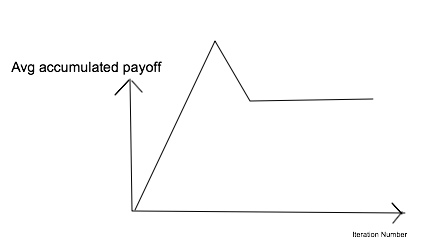
\includegraphics[width=0.4\textwidth,center]{images/like-similarity-dg} \caption{Expected payoff in
%		 peer-like-similarity strategy}

%\end{center} \end{figure}


\paragraph{} In the case of having mixed number of
peers that half of them use random strategy and the other half use peer-like-similarity
strategy, we expect the average accumulated payoff to have a slope
more moderate than in peer-like-similarity strategy but steeper than
in  random strategy while the value of average accumulated payoff is
increasing. 

%\begin{figure}[h!] \begin{center}
%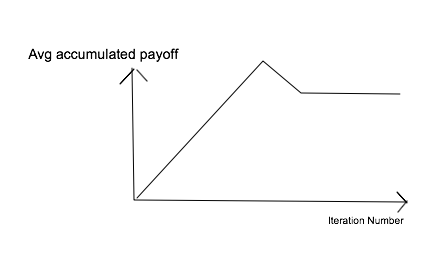
\includegraphics[width=0.4\textwidth,center]{images/mix-dg}
%\caption{Expected payoff when both strategies} \end{center} \end{figure}


\subsubsection{Settings}

he simulation metrics and their values within the experiment are as the following.


\begin{table}[h!]
\caption{Agent types and population}
\begin{center}
\begin{tabular}{cc}


\begin{tabular}{|c|c|}
\hline

\# of Document &  400  \\ \hline
Total \# of peers & 50 \\ \hline		
\# of consumer peers & 50 \\ \hline 
\#of producer peers & 0 \\ \hline

\end{tabular}

&


\begin{tabular}{|c|c|}
\hline

Memory-based & yes   \\ \hline
K   & 5 \\ \hline
\# of iterations & 160 \\ \hline		
\end{tabular}

\end{tabular}
\end{center}
\label{default}
\end{table}



\begin{table}[h!]
\caption{Document tags and peer's tastes}

\begin{center}

\begin{tabular}{|c|c|}
\hline tag/taste values & (0 1 )\\
\hline \# of document tags   &  1\\ \hline 
\# of peer tastes  &  1 \\ \hline 
\end{tabular}

\end{center}
\label{default}
\end{table}

\subsubsection{Results and Discussion}

\begin{figure}[h!] \begin{center}
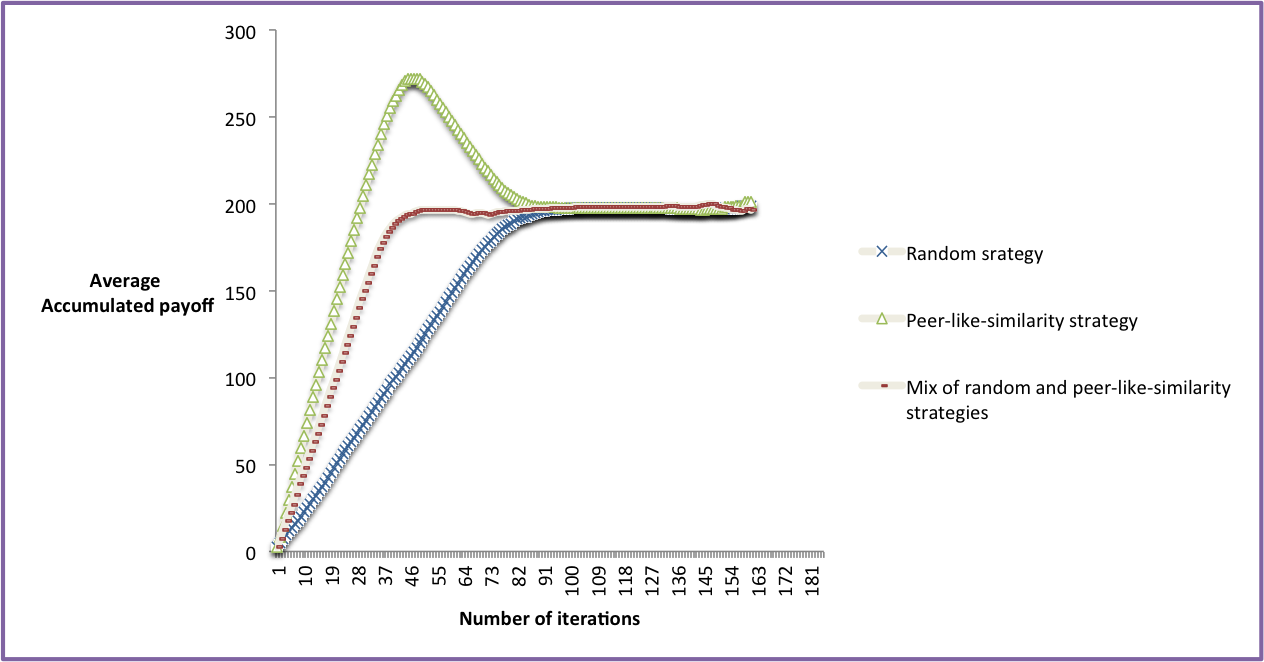
\includegraphics[width=0.6\textwidth,center]{images/randSimMix}
\caption{Average accumulated payoff for Random and Peer-like-similarity strategies} \end{center} \end{figure}

The result of simulations for the two strategies, and mix of the strategies are depicted into the diagram  below.
As we expected in our hypotheses, in Random strategy the average accumulated payoff constantly increased by a relatively low sheer until all
the documents were visited by the peers. However, in peer-like-similarity the growth of average accumulated payoff was faster than random strategy, 
but, it started decreasing after some point in simulation until all the documents were visited. 

In the case of running the simulation with mix strategy, half of the peers using random strategy and the other half using peer-like-similarity strategy, the rate of
growth of average accumulated payoff was between the rate of growth in the two strategies and the rate of growth never got negative. 


\subsection{Experiment 2}

\subsubsection{Goal}The impact of number of tags on average accumulated payoff in random and peer-like-similarity strategies.

%the metric values: \newline number existing tags and tastes: 2
%when (\#taste for each peer =1 and \#tags for each document=1)
%\newline number existing tags and tastes: 8 when (\#taste for each
%peer =3 and \#tags for each document=2)

\subsubsection{Hypothesis} 

\paragraph{}
In random strategy, when the number of existing tags are
increasing, we expect a lower probability of a document to be liked by each peer.
When a document d has one attached tag
and the set of existing tags are \{T1, T2\},

$\Pr({like(p, d)}) = \frac{1}{2} $
\newline\newline And, when a document d has one attached tag and the set of
existing tags are \{T1, T2, T3, T4, T5, T6\}:

$\Pr({like(p, d)}) = \frac{1}{6} $

%\paragraph{} And, in general $\Pr(p, d)$ in random strategy can be
%	calculated as
%
%		$$\Pr^{random}(p, d) = \sum _{i=1} ^{NAT}  \frac{1}{NET} $$
%
%		where NAT is the number of attached tags, and NET is the
%	number of existing tags. 

\paragraph{} However, Increasing the number of tags will not affect on the performance of peer-like-similarity strategy substantially.
Since when the number of common document likes between two peers increases in to a level that they cover all the tastes attached to each peer,
we can be certain that the searching peer would like any unvisited document that the other peer was previously liked.  


\subsubsection{Settings}

The simulation metrics and their values within the experiment are as the following.

\begin{table}[h!]
\caption{Agent types and population}

\begin{center}

\begin{tabular}{cc}

\begin{tabular}{|c|c|}
\hline

\# of Document &  400  \\ \hline
Total \# of peers & 100 \\ \hline		
\# of consumer peers & 100 \\ \hline 
\#of producer peers & 0 \\ \hline

\end{tabular}

&

\begin{tabular}{|c|c|}
\hline
Memory-based & yes   \\ \hline
K   & 5 \\ \hline
\# of iterations & 160 \\ \hline		
\end{tabular}


\end{tabular}

\end{center}
\label{default}
\end{table}


\begin{table}[h!]
\caption{Document tags and Peer tastes}

\begin{center}

\begin{tabular}{cc}

\begin{tabular}{|c|c|}
\hline tag/taste values & (0 1)\\
\hline \# of document tags  &  1\\ \hline 
\# of peer tastes  &  1 \\ \hline 
\end{tabular}

&

\begin{tabular}{|c|c|}
\hline tag/taste values & (0 1 2 )\\
\hline \# of document tags   &  1\\ \hline 
\# of peer tastes  &  1 \\ \hline 
\end{tabular}


\\ \\

\begin{tabular}{|c|c|}
\hline tag/taste values & (0 1 2 3)\\
\hline \# of document tags   &  1\\ \hline 
\# of peer tastes  &  1 \\ \hline 
\end{tabular}



\end{tabular}

\end{center}
\label{default}
\end{table}

\subsubsection{Results and Conclusion}


\begin{figure}[bp!]
\begin{center}
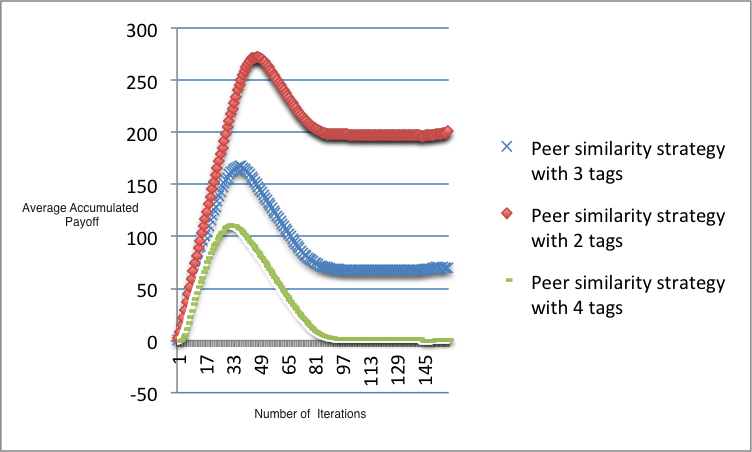
\includegraphics[width=0.6\textwidth,center]{images/SimTags}
\caption{Peer-like-similarity strategy with different number of tags}
\label{fig:images/EXP2-1}
\end{center}
\end{figure}

\begin{figure}[bp!]
\begin{center}
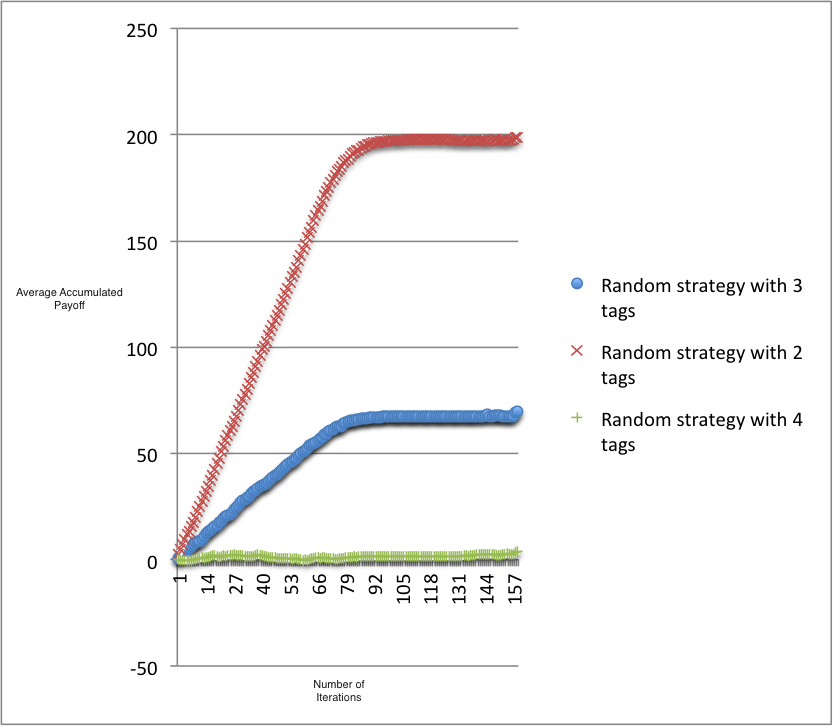
\includegraphics[width=0.6\textwidth,center]{images/RandTags}
\caption{Random strategy with different number of tags}
\label{fig:images/EXP2-2}
\end{center}
\end{figure}


As we expected from our hypotheses, the average accumulated payoff decreased dramatically in random strategy when the number of existing tags were increased.
But, In peer-like-similarity the slop of changes remained fixed in the the three experiments and only a constant negative shift of average accumulated payoff
was observed. 



\subsection{Experiment 3}

\subsubsection{Goal} Comparison of peer-follow-similarity strategy with peer-distance-similarity strategy based on accumulated peer payoff. 

\subsubsection{Hypothesis}


Let's consider the case where P1 likes \{d1,d2,d3\}, P2 likes
 \{d2,d3,d4\}, and P3 likes  \{d4,d5,d6\}. Also, P1 follows P2 and P2 Follows P3.
 In order to return relevant documents to P1, peer-like-similarity and peer-follow-similarity strategies will not return d4 as a relevant document.
But, d4 can be returned as relevant in peer-distance strategy based on the distance metric between the searching peer and the peers who liked the document d4.

However, after a number of turns, when each peer starts following other peers, the documents that a peer is going to like could be liked by one or more of the following peers.
In this condition, peer-follow-similarity would outperform peer-distance strategy as it considers the similarity level of 
following peers while in distance strategy, all the following peers will have the same distance of (distance = 1) and have equal effect in ranking documents.
%
%
%Probability of P1 like d6:  probability(P2, d6) * similarity(p1, p2)  
%Probability of P1 like d4:  similarity(P1, p2).
%
%However, in  peer-like-similarity:
%similarity(P1, P3)  is not defined. 
%indirect similarity relation of peers to each other.

\subsubsection{Settings}


The simulation metrics and their values within the experiment are as the following.

\begin{table}[h!]
\caption{Agent types and population}
\begin{center}
\begin{tabular}{cc}


\begin{tabular}{|c|c|}
\hline

\# of Document &  400  \\ \hline
Total \# of peers & 50 \\ \hline		
\# of consumer peers & 50 \\ \hline 
\#of producer peers & 0 \\ \hline

\end{tabular}

&


\begin{tabular}{|c|c|}
\hline

Memory-based & yes   \\ \hline
K   & 5 \\ \hline
\# of iterations & 160 \\ \hline		
\end{tabular}

\end{tabular}
\end{center}
\label{default}
\end{table}



\begin{table}[h!]
\caption{Document tags and peer's tastes}

\begin{center}

\begin{tabular}{|c|c|}
\hline tag/taste values & (0 1 )\\
\hline \# of document tags   &  1\\ \hline 
\# of peer tastes  &  1 \\ \hline 
\end{tabular}

\end{center}
\label{default}
\end{table}





\subsubsection{Results and Conclusion}

The peer distance and peer follow strategy resulted in the same slope and similar values of 
average accumulated payoff during the interactions of peers. This result indicate that after a small number of
interactions, the peers, who are interested in each other, the followed peers, are identified. 
After that point,the documents that are returned in the topK of the peers are previously liked by followers of each searching peer. 


\begin{figure}[h!]
\begin{center}
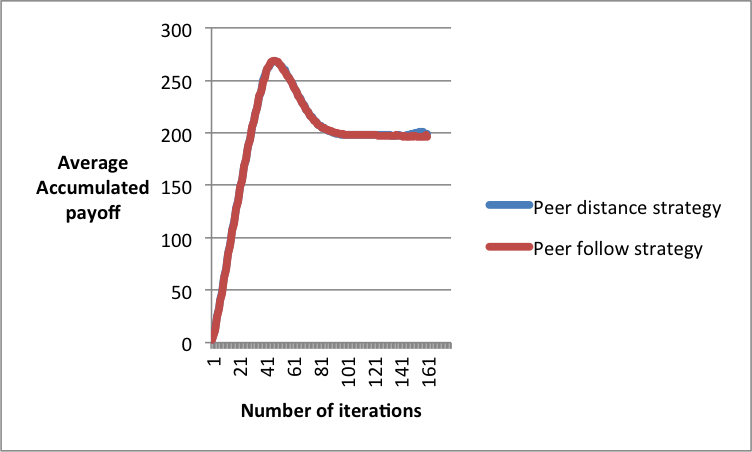
\includegraphics[width=0.6\textwidth,center]{images/distance-follow}
\caption{The average accumulated payoff in peer-distance and peer-follow strategies}
\label{fig:images/EXP3-2}
\end{center}
\end{figure}


\subsection{Experiment 4}
\subsubsection{Goal}
 Study the relationship of average accumulated payoff with the number of iterations  in random and document-popularity strategies.
\subsubsection{Hypothesis}

\begin{itemize}
\item Random Strategy performance: The reasoning on the performance of random strategy was explained in the previous section.

\item Document-popularity strategy performance: Given that half of the peers have taste 0, and the other half of the peers have taste 1,
a popular document that is liked by any subset of each half, would be liked only by the other members of that half. 

Therefore, if there are peers who have distinct taste, the document popularity would be useful only when peers of the same taste have made 
that document popular. On the other side, when the majority of peers have common tastes in a network, the most popular documents are liked by
a subset of peers which their majority have common tastes. 

Thus, we can divide the peers of a network in two groups. Peers with minor tastes and peer with major tastes.
Peers with major tastes would benefit the most from document popularity strategy, while peers with minor tastes would benefit the least since 
those documents are liked and got popular by the peers which most of them have the major taste.


since $ |Peer_{minor} |\ <\ |peer_{major}| $, Assuming that a popular document is liked by a group of peers $P$ where ${ p \in P}$. Since
$ \Pr(|p_{major}| > |p_{minor}|) > \Pr(|p_{major}| < |p_{minor}|)$ , then  $Pr(P_{minor}\ like\  the\ popular-document\ d\ )  < Pr(P_{major}\ like\  the\ popular-document\ d\ )     $
 
\end{itemize}

\subsubsection{Experiment Settings}

The simulation metrics and their values within the experiment are as the following.


\begin{table}[h!]
\caption{Document filtering strategies}
\begin{center}

\begin{tabular}{cc}


\begin{tabular}{|c|c|}
\hline Ranking Strategy & Memory-based\\
\hline Random strategy  &  yes\\ \hline 
Document-popularity strategy  &  yes \\ \hline 
\end{tabular}


&


\begin{tabular}{|c|c|}
\hline
K   & 5 \\ \hline
\# of iterations & 160 \\ \hline		
\end{tabular}


\end{tabular}
\end{center}
\label{default}
\end{table}



\begin{table}[h!]
\caption{Agent types and population}
\begin{center}

\begin{tabular}{|c|c|}
\hline

\# of Document &  400  \\ \hline
Total \# of peers & 50 \\ \hline		
\# of consumer peers & 50 \\ \hline 
\#of producer peers & 0 \\ \hline

\end{tabular}

\end{center}
\label{default}
\end{table}






\begin{table}[h!]
\caption{Document tags and peer's tastes}

\begin{center}

\begin{tabular}{|c|c|}
\hline tag/taste values & (0 1 )\\
\hline \# of document tags   &  1\\ \hline 
\# of peer tastes  &  1 \\ \hline 
\end{tabular}

\end{center}
\label{default}
\end{table}


\subsubsection{Result And Discussion}

\begin{figure}[h!]
\begin{center}
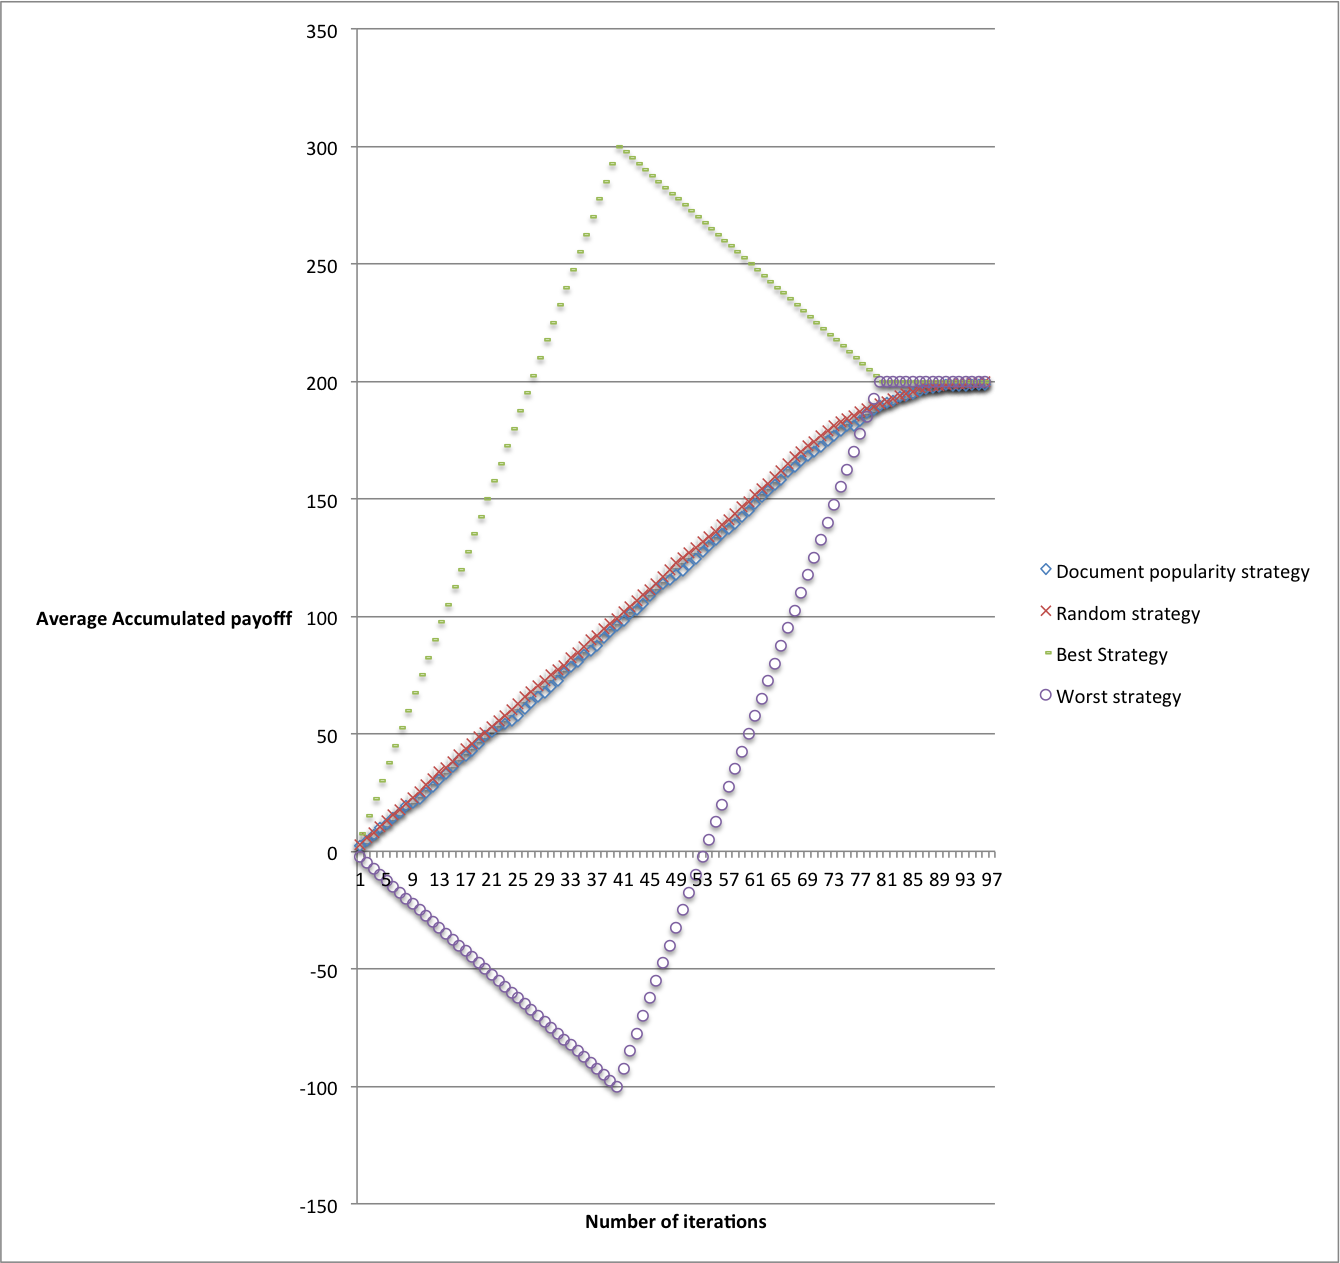
\includegraphics[width=0.6\textwidth,center]{images/doc-pop-rand-2taste}
\caption{The average accumulated payoff in document-popularity and random strategies}
\label{fig:images/EXP3-2}
\end{center}
\end{figure}

 In the presence of uniform tastes and tags for peers and documents, 
there were in fact no major or minor tastes in the network and the average accumulated payoff slop was the same as in random strategy. 

\begin{figure}[h!]
\begin{center}
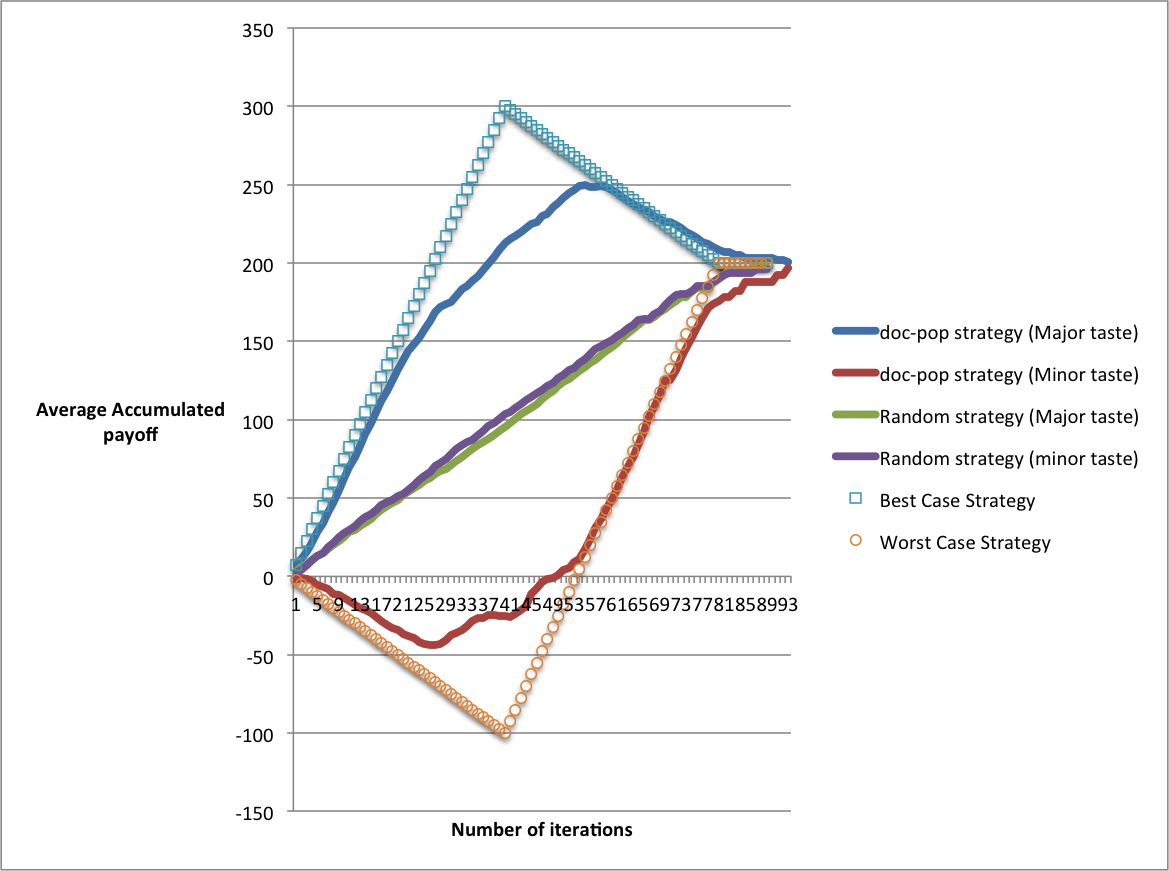
\includegraphics[width=0.6\textwidth,center]{images/Exp4-doc-pop-and-random-MajorMinor}
\caption{The average accumulated payoff in document-popularity and random strategies in the presence of Minor and Major tastes}
\label{fig:images/EXP3-2}
\end{center}
\end{figure}

In the presence of producers with major and minor tastes, the result showed that minor or major tastes of producers does not affect the 
payoff of individuals in random strategy. But, The performance of producers with minor tastes and producers with major tastes crucially differed when they were using document-popularity
strategy. And, the producers with Major taste had a a higher accumulated payoff in compared with producers with minor taste. 




\subsection{Experiment 5}
\subsubsection{Goal}
 Study the relationship of average accumulated payoff with the number of iterations  in peer-popularity and peer-like-similarity strategies
\subsubsection{Hypothesis}

\begin{itemize}

\item Peer-like-similarity strategy:
we explained on the behaviour of peer-like-similarity strategy before. 

\item Peer-popularity strategy: 

Followers of a peer are those who have similar taste with that peer. 
when  documents are ranked with peer-popularity. And in Peer popularity strategy, documents get sorted by the number of followers of peers who like a document.

The number of followers in fact, represents the number of peers who previously liked at least one of the documents that the searching peer has liked. 

In every document search, if returned documents are ranked by the peer-popularity strategy and give that there are two groups of peers each with distinct tastes,
the  strategy would do the ranking based on peers with the most number of followers, which can have either of these two distinct tastes. 
Therefore, we can assume the chance of a document being liked would equal $\frac{1}{|peer-groups-with-distinict-tastes|} $.

\end{itemize}

\subsubsection{Experiment Settings}

The simulation metrics and their values within the experiment are as the following.

\begin{table}[h!]
\caption{Document filtering strategies}
\begin{center}

\begin{tabular}{cc}


\begin{tabular}{|c|c|}
\hline Ranking Strategy & Memory-based\\
\hline Peer-popularity  &  yes\\ \hline 
Peer-like-similarity  &  yes \\ \hline 
\end{tabular}

&

\begin{tabular}{|c|c|}
\hline
K   & 5 \\ \hline
\# of iterations & 80 \\ \hline		
\end{tabular}


\end{tabular}
\end{center}
\label{default}
\end{table}


\begin{table}[h!]
\caption{Agent types and population}
\begin{center}

\begin{tabular}{|c|c|}
\hline

Total \# of Documents &  400  \\ \hline
\# of Documents with tag 0 &  200  \\ \hline
\# of Documents with tag 1 &  200  \\ \hline

Total \# of peers & 50 \\ \hline	
	
\# of consumer peers with taste 0  & 25 \\ \hline
\# of consumer peers with taste 1  & 25 \\ \hline 

\#of producer peers & 0 \\ \hline

\end{tabular}

\end{center}
\label{default}
\end{table}




\begin{table}[h!]
\caption{Document tags and peer's tastes}

\begin{center}

\begin{tabular}{|c|c|}
\hline tag/taste values & (0 1 )\\
\hline \# of document tags   &  1\\ \hline 
\# of peer tastes  &  1 \\ \hline 
\end{tabular}

\end{center}
\label{default}
\end{table}


\subsubsection{Discussion and Results}

The result of experiment showed outperformance of peer-similarity strategy over peer-popularity strategy. 
This could be justified with our hypothese on peer-similarity strategy in that in the presence of two
group of peers with distinct tastes, the peer-popularity strategy would act similar to random strategy. And the probability
of each document being liked would be $\frac{1}/{2}$.  

\begin{figure}[h!]
\begin{center}
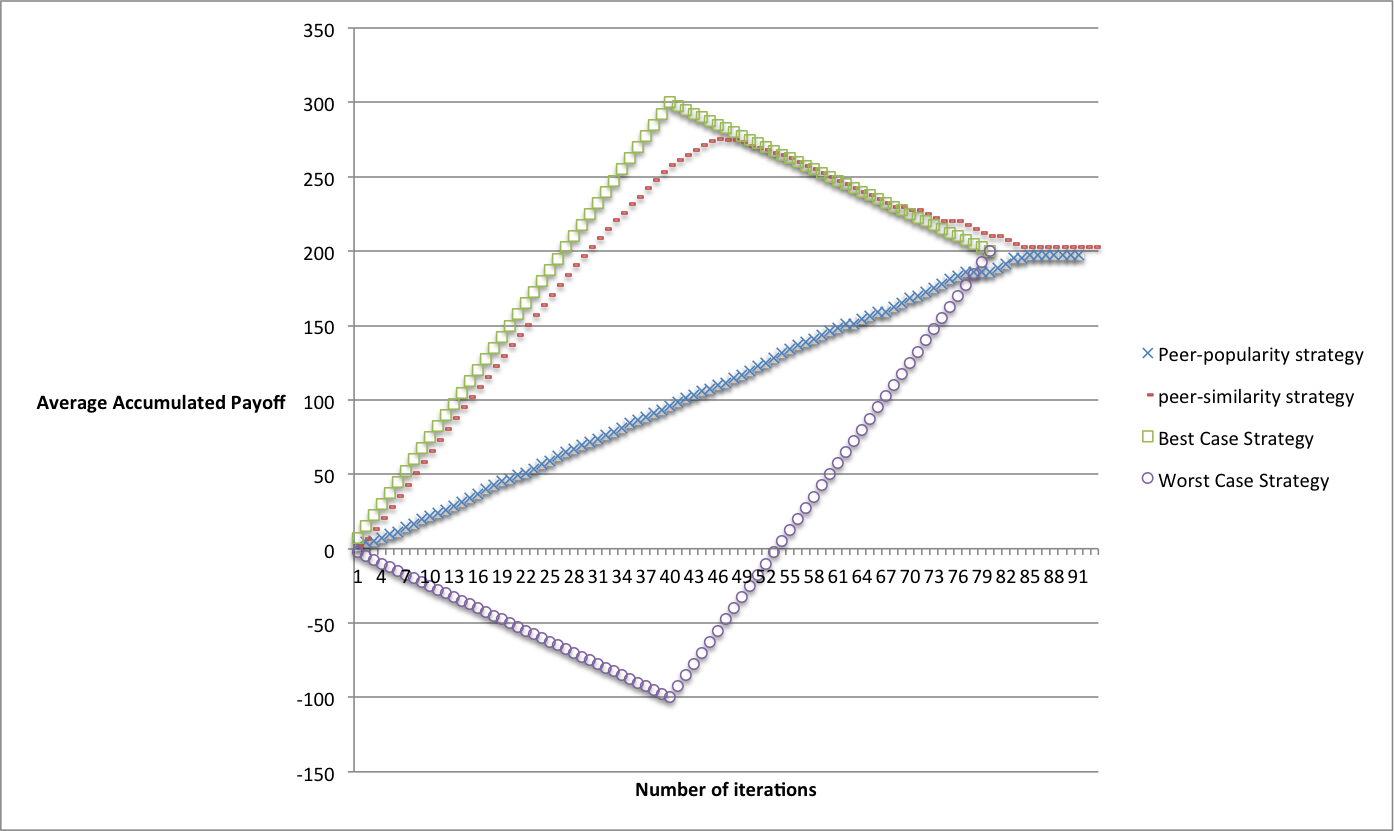
\includegraphics[width=0.6\textwidth,center]{images/peer-pop-peer-sim-2taste}
\caption{Average accumulated payoff with the number of iterations in peer-popularity and peer-like-similarity strategies}
\label{fig:images/EXP3-2}
\end{center}
\end{figure}

In the presence of Major and minor taste consumers, the result of experiment was similar to the above expriment when the taste of
consumers were uniform. The producers with minor taste in peer\-like\-similarity strategy outperformed the Major and Minor producers that used peer-popularity
strategy. 

peer-similarity strategy over peer-popularity strategy. 
This could be justified with our hypothese on peer-similarity strategy in that in the presence of two
group of peers with distinct tastes, the peer-popularity strategy would act similar to random strategy. And the probability
of each document being liked would be $\frac{1}{2}$.  


\begin{figure}[h!]
\begin{center}
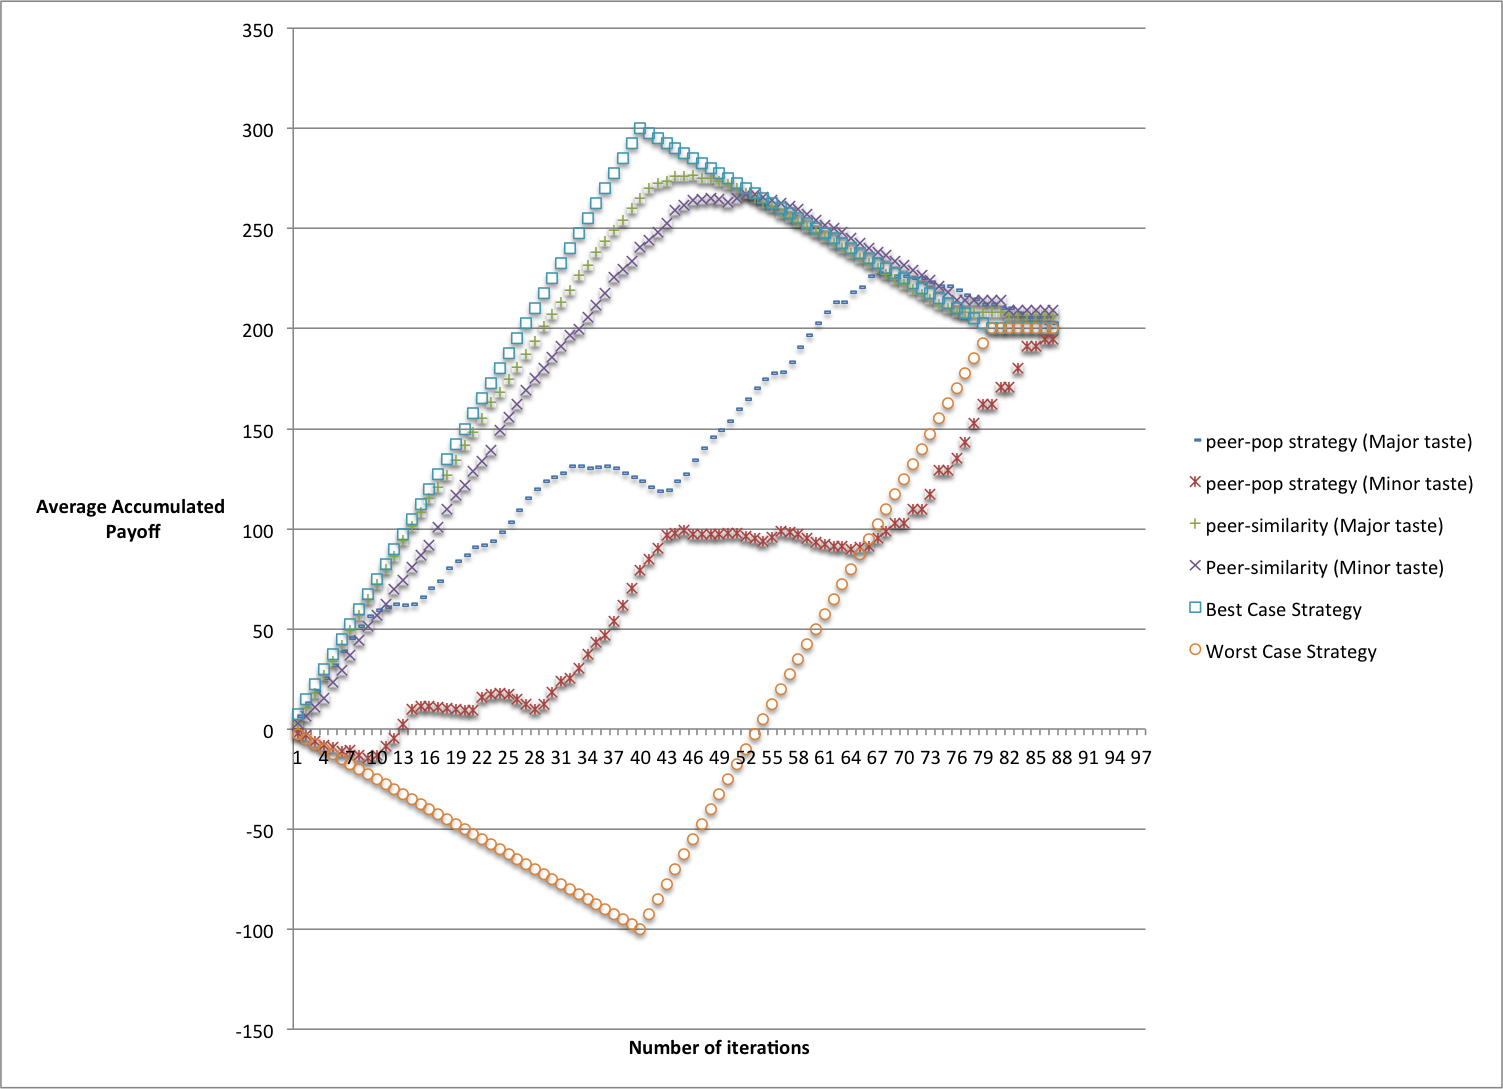
\includegraphics[width=0.6\textwidth,center]{images/Exp4-peer-pop-and-peer-sim-MajorMinor}
\caption{Average accumulated payoff with the number of iterations in peer-popularity and peer-like-similarity strategies in the presence of Minor and 
Major tastes}
\label{fig:images/EXP3-2}
\end{center}
\end{figure}

\subsection{Experiment 6}
\subsubsection{Goal}
Study the performance of producers and consumers with minor and major tastes when both producer and consumer use document-popularity strategy.
\subsubsection{Hypothesis}

	\begin{itemize}

	\item When the producer and the consumer  both have the major
taste: we should expect depending on the strategy the consumer is
using, that strategy would choose the published document in its topK
sooner than the non-relavent documents to that consumer. And
selection of those documents would lead to the increase of payoff of
the publishers.

	Once the peers visited all the documents including the published
ones, the payoff of each publisher would be equal to  $ {number\ of\
published\ documents} * {the\ number\ of\ consumers\ with\ similar\
tastes\ of\ the\ producer} $


	And we can predict the payoff of publishers, for each iteration
as:

	``The number of consumer peers that choose that document in their
topK''

	When producer and consumer both are using document popularity
strategy, the strategy would rank documents based on the number of
peers who liked the documents, Therefore, the documents that are in
in the interest of the major of number of peers, ( have the major
taste) would be ranked as the highest documents. We expect the payoff
a producer and consumer that have the minor taste, would be lower
than the payoff of a producer and consumer that have a major taste
respectively.




	\item When the producer and the consumer both have minor taste:
We expect that document popularity strategy would not place the minor
taste documents into TopK in the beginning of the experiment untill
it runs out of documents that are in the interest of peers of peers
with major tastes. In the presence of peers with minor and major
tastes, a random strategy would be the most useful, since it randomly
picks the documents with different tastes in the topk.

	\end{itemize}

\subsubsection{Experiment Settings}

The simulation metrics and their values within the experiment are as the following.

\begin{table}[h!]
\caption{Document filtering strategies}
\begin{center}

\begin{tabular}{cc}


\begin{tabular}{|c|c|}
\hline Ranking Strategy & Memory-based\\
\hline document-popularity  &  yes\\ \hline 
\end{tabular}

&

\begin{tabular}{|c|c|}
\hline
K   & 5 \\ \hline
\# of iterations & 110 \\ \hline		
\end{tabular}


\end{tabular}
\end{center}
\label{default}
\end{table}


\begin{table}[h!]
\caption{Agent types and population}
\begin{center}


\begin{tabular}{|c|c|}
\hline

Total \# of Documents &  400  \\ \hline
\# of Documents with tag 0 &  200  \\ \hline
\# of Documents with tag 1 &  200  \\ \hline

Total \# of peers & 60 \\ \hline
\# of producer peers with taste 1  & 21 \\ \hline
\# of producer peers with taste 0  & 9 \\ \hline 

\#of consumer peers with taste 1 & 21 \\ \hline
\#of consumer peers with taste 0 & 9 \\ \hline

\end{tabular}


\end{center}
\label{default}
\end{table}


\begin{table}[h!]
\caption{Document tags and peer's tastes}

\begin{center}

\begin{tabular}{|c|c|}
\hline tag/taste values & (0 1 )\\
\hline \# of document tags   &  1\\ \hline 
\# of peer tastes  &  1 \\ \hline 
\end{tabular}

\end{center}
\label{default}
\end{table}


\subsubsection{Discussion and Results}

The experiment was done in the presence of major and minor taste producers and consumers. 

The impact of document popularity strategy on the performance of producer payoff showed that producers and consumers of major tastes  had a higher average accumulated payoff 
in compared with producers and consumers with minor tastes.  

   
\begin{figure}[h!]
\begin{center}
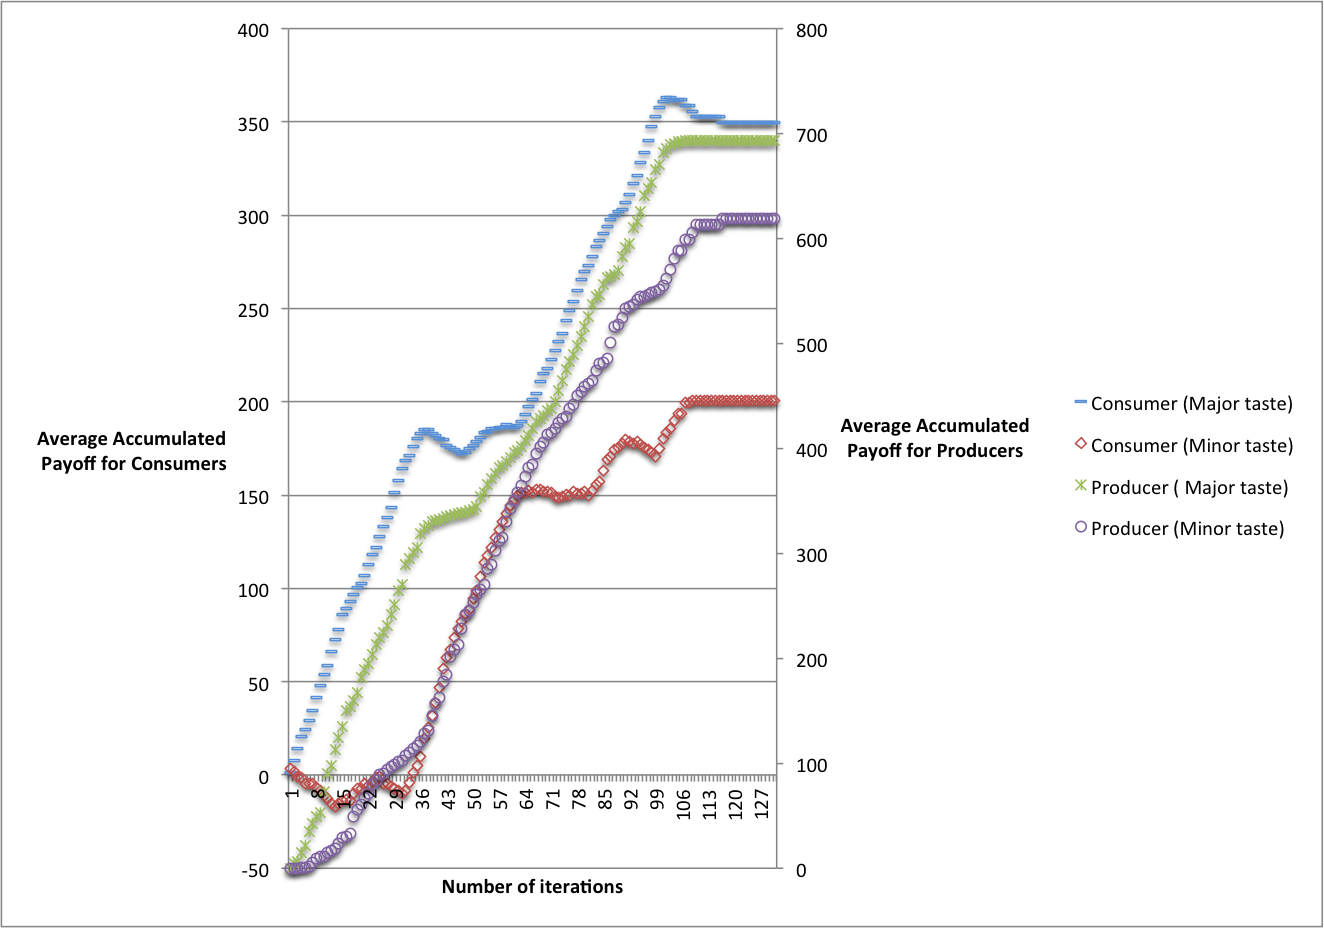
\includegraphics[width=0.6\textwidth,center]{images/EXP7-Doc-pop-prod-cons}
\caption{Performance of producers with tag 0 and tag 1 when different portion of consumers have different tastes}
\label{fig:images/EXP3-2}
\end{center}
\end{figure}


\subsection{Experiment 7}
\subsubsection{Goal}
Study the performance of producers and consumers with minor and major tastes when both producer and consumer use random strategy.
\subsubsection{Hypothesis}

When the consumers and producers use random strategy, the selection of topK documents follows a random order.
Therefore, the taste of consumers and producers will not have any effect in performance of the producers and consumers. 

\subsubsection{Experiment Settings}

The simulation metrics and their values within the experiment are as the following.

\begin{table}[h!]
\caption{Document filtering strategies}
\begin{center}

\begin{tabular}{cc}


\begin{tabular}{|c|c|}
\hline Ranking Strategy & Memory-based\\
\hline Random strategy  &  yes\\ \hline 
Document popularity strategy  &  yes \\ \hline 
\end{tabular}

&

\begin{tabular}{|c|c|}
\hline
K   & 5 \\ \hline
\# of iterations & 110 \\ \hline
\end{tabular}


\end{tabular}
\end{center}
\label{default}
\end{table}


\begin{table}[h!]
\caption{Agent types and population}
\begin{center}


\begin{tabular}{|c|c|}
\hline

Total \# of Documents &  400  \\ \hline
\# of Documents with tag 0 &  200  \\ \hline
\# of Documents with tag 1 &  200  \\ \hline

Total \# of peers & 60 \\ \hline
\# of producer peers with taste 1  & 21 \\ \hline
\# of producer peers with taste 0  & 9 \\ \hline 

\#of consumer peers with taste 1 & 21 \\ \hline
\#of consumer peers with taste 0 & 9 \\ \hline

\end{tabular}


\end{center}
\label{default}
\end{table}



\begin{table}[h!]
\caption{Document tags and peer's tastes}

\begin{center}

\begin{tabular}{|c|c|}
\hline tag/taste values & (0 1 )\\
\hline \# of document tags   &  1\\ \hline 
\# of peer tastes  &  1 \\ \hline 
\end{tabular}

\end{center}
\label{default}
\end{table}

\subsubsection{Discussion and Results}
As it was predicted in our hypotheses, in the presence of random strategy, the topK were selected randomly regardless of the minor taste or major taste of producers and consumers. 
  
In the experiment, the consumers with major taste ended visiting all their document with a higher average accumulated payoff since 70 percent of published documents were in the interest of consumers with major tastes. 


\begin{figure}[h!]
\begin{center}
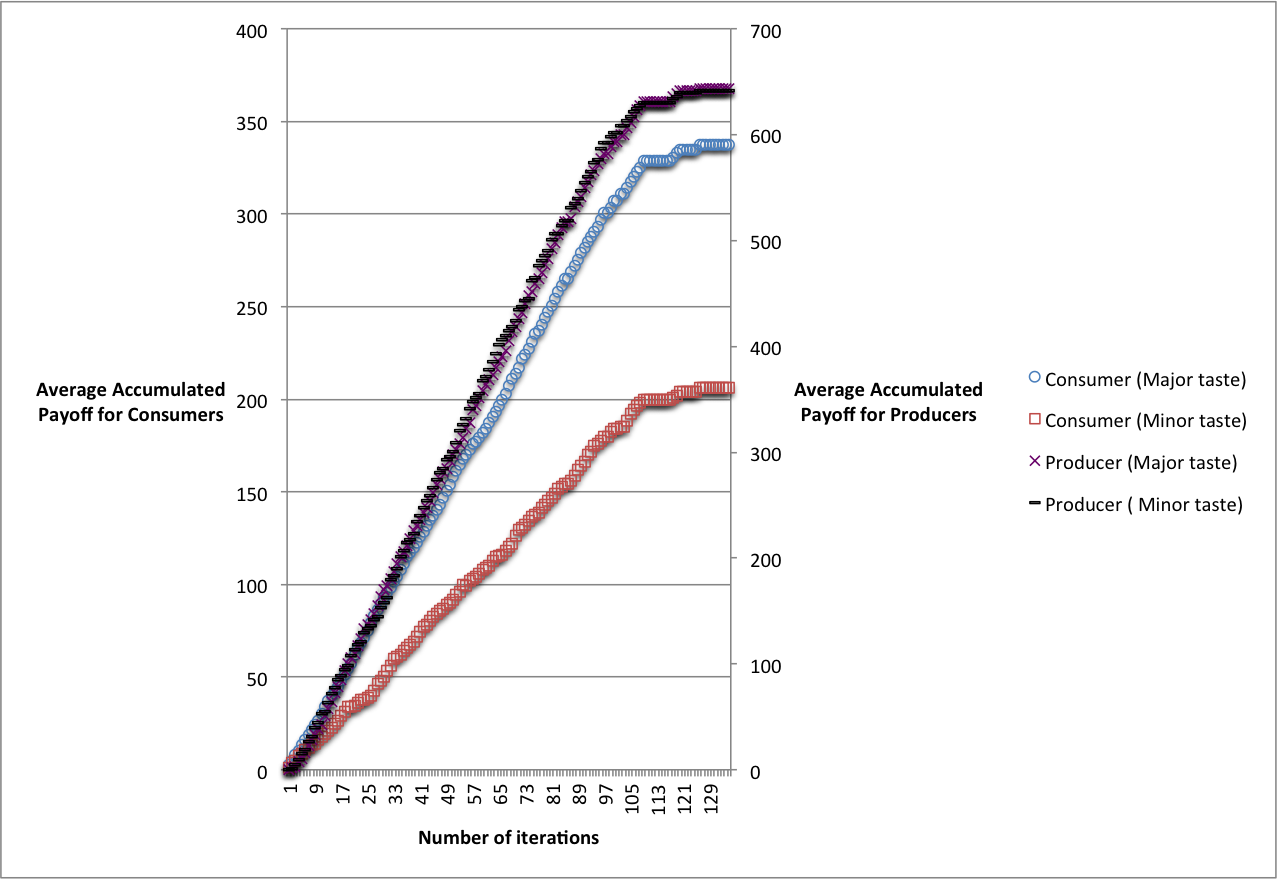
\includegraphics[width=0.6\textwidth,center]{images/EXP6-RandomStrategy-prod-cons}
\caption{Performance of producers with tag 0 and tag 1 when different portion of consumers have different tastes}
\label{fig:images/EXP3-2}
\end{center}
\end{figure}


\subsection{Experiment 8}
\subsubsection{Goal}
Comparison of the performance of producers and consumers with minor and major tastes for three different strategies of peer-like-similarity, Random, and 
Document popularity.  

\subsubsection{Hypothesis}

When consumers use peer-like-similarity strategy, the documents are ranked by the number of common document likes between the searching peer and other peers.
In the presence of producers, when a document is published, initially, there would be not document like,and there would be less number of document likes
in compared with existing documents. The average accumulated payoff of the producer would be the least amount, when the producer has a minor taste, and publishes
documents. Therefore, a document being of a minor taste, and the the document being recently published and not being visited and liked by many peers would 
both affect the producer payoff in peer-like-similarity strategy.   

The hypothesis for the two other strategies of random and document-popularity was discussed separtely in  


\subsubsection{Experiment Settings}

The simulation metrics and their values within the experiment are as the following.

\begin{table}[h!]
\caption{Document filtering strategies}
\begin{center}

\begin{tabular}{cc}


\begin{tabular}{|c|c|}
\hline Ranking Strategy & Memory-based\\
\hline Document-popularity  &  yes\\ \hline 
Peer-like-similarity  &  yes \\ \hline 
Random  &  yes \\ \hline 
\end{tabular}

&

\begin{tabular}{|c|c|}
\hline
K   & 5 \\ \hline
\# of iterations & 110 \\ \hline
\end{tabular}


\end{tabular}
\end{center}
\label{default}
\end{table}


\begin{table}[h!]
\caption{Agent types and population}
\begin{center}


\begin{tabular}{|c|c|}
\hline

Total \# of Documents &  400  \\ \hline
\# of Documents with tag 0 &  200  \\ \hline
\# of Documents with tag 1 &  200  \\ \hline

Total \# of peers & 60 \\ \hline
\# of producer peers with taste 1  & 21 \\ \hline
\# of producer peers with taste 0  & 9 \\ \hline 

\#of consumer peers with taste 1 & 21 \\ \hline
\#of consumer peers with taste 0 & 9 \\ \hline

\end{tabular}


\end{center}
\label{default}
\end{table}



\begin{table}[h!]
\caption{Document tags and peer's tastes}

\begin{center}

\begin{tabular}{|c|c|}
\hline tag/taste values & (0 1 )\\
\hline \# of document tags   &  1\\ \hline 
\# of peer tastes  &  1 \\ \hline 
\end{tabular}

\end{center}
\label{default}
\end{table}


\subsubsection{Discussion and Results}

%\begin{figure}[h!]
%\begin{center}
%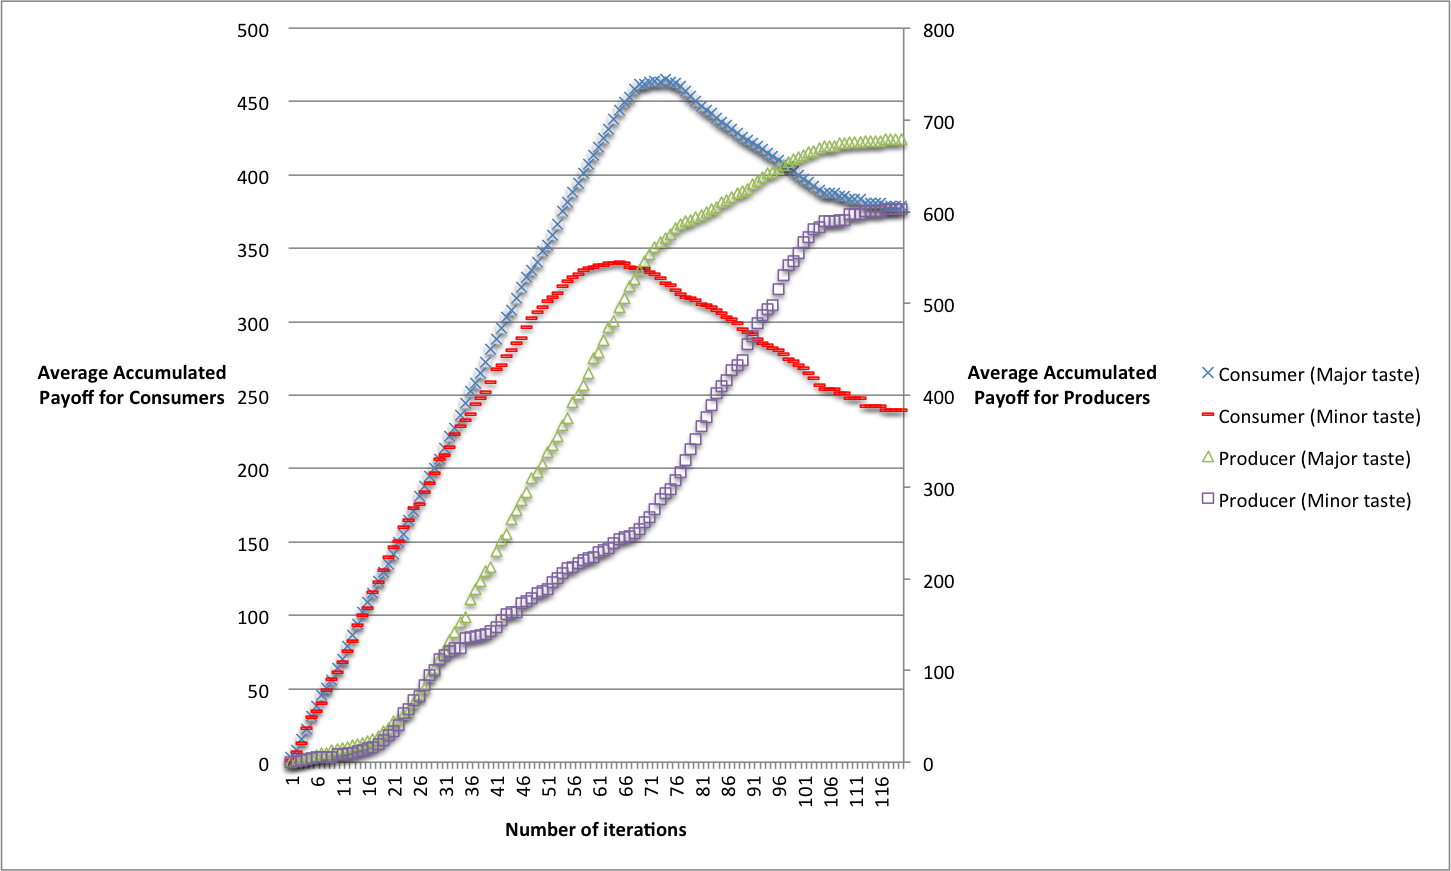
\includegraphics[width=0.6\textwidth,center]{images/EXP9-Peerlike-simi-prod-cons}
%\caption{Performance of producers with tag 0 and tag 1 when different portion of consumers have different tastes}
%\label{fig:images/EXP3-2}
%\end{center}
%\end{figure}


In Figure \ref{fig:images/F11}, the performance of producers with Major taste shows the average accumulated payoff in $ document-popularity > random > peer-like-similarity$
in the first half of the interactions, and the average accumulated payoff of $ peer-like-sim > random > Document-popularity$ in
the second half of the interactions.  


\begin{figure}[h!]
\begin{center}
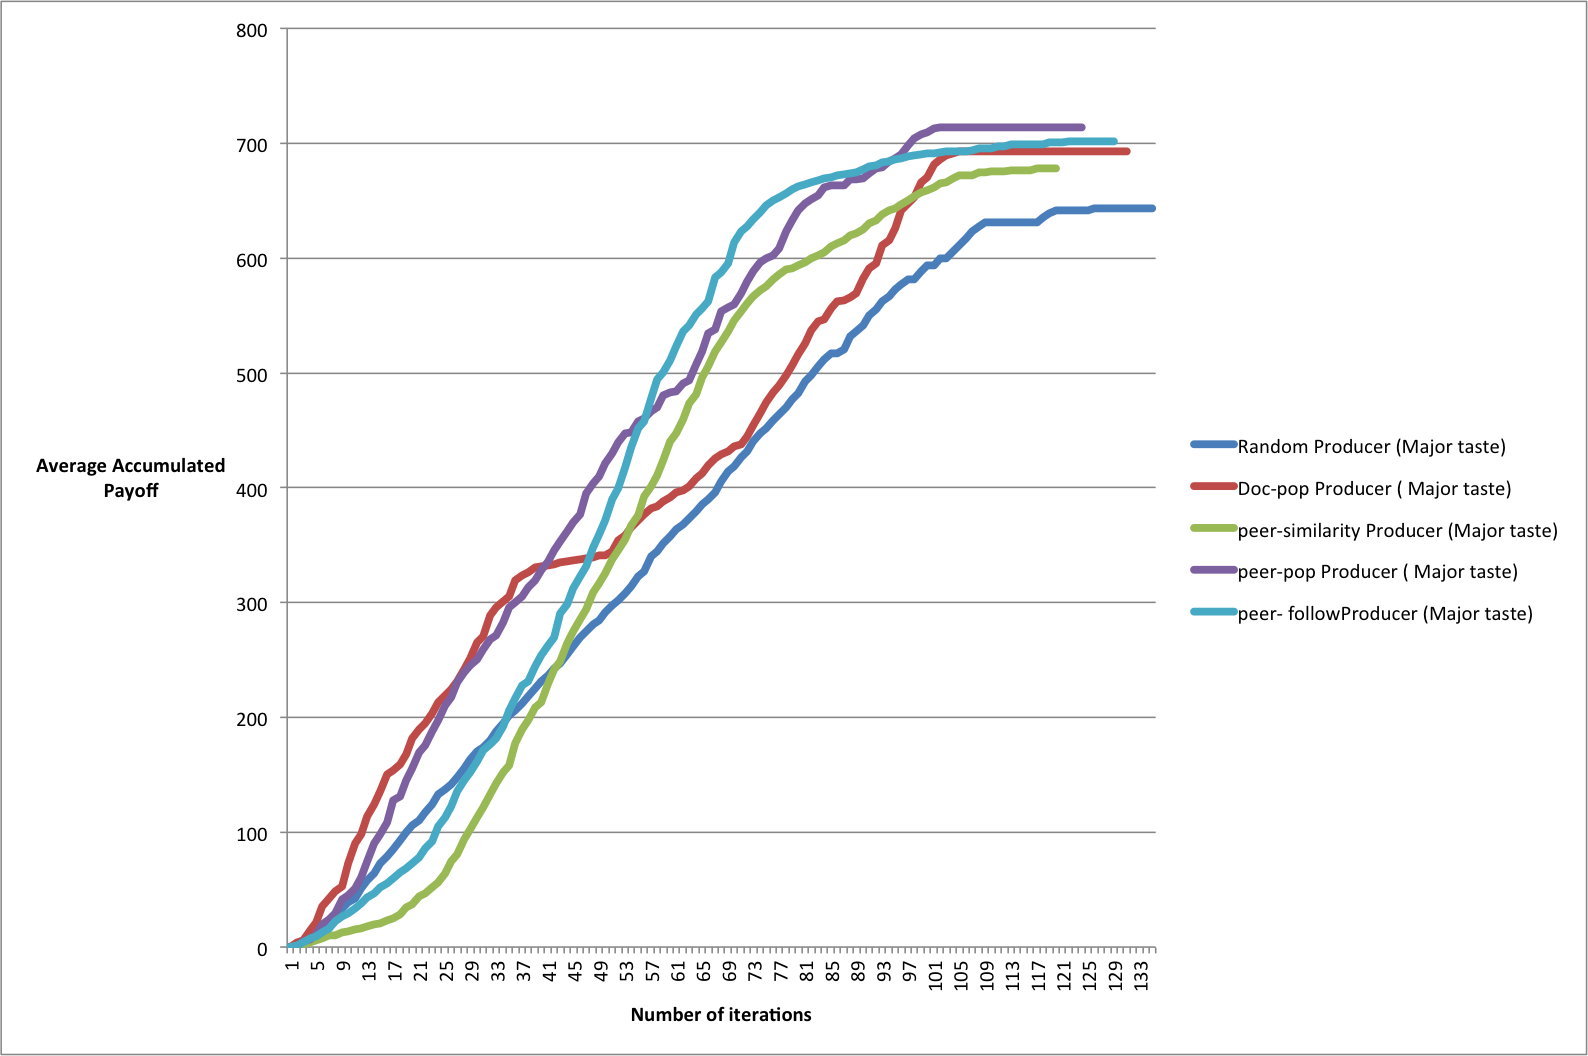
\includegraphics[width=0.6\textwidth,center]{images/EXP8-Strategies_Prod-Major-taste}
\caption{Producers with major taste}
\label{fig:images/F11}
\end{center}
\end{figure}

In  Figure \ref{fig:images/F12} the performance of producers with minor taste shows the average accumulated payoff in $  random > Document-popularity > peer-like-similarity$.  
%The reason that document-popularity outperformed peer-like-similarity strategy, was the the number of documents with their tag value equal to minor taste,
%was  $200+ 9 * 5 =  245$ while the number of peers with minor taste were 30 percent of the whole population of peers, which is $ 60 * 0.3 = 18 $


\begin{figure}[h!]
\begin{center}
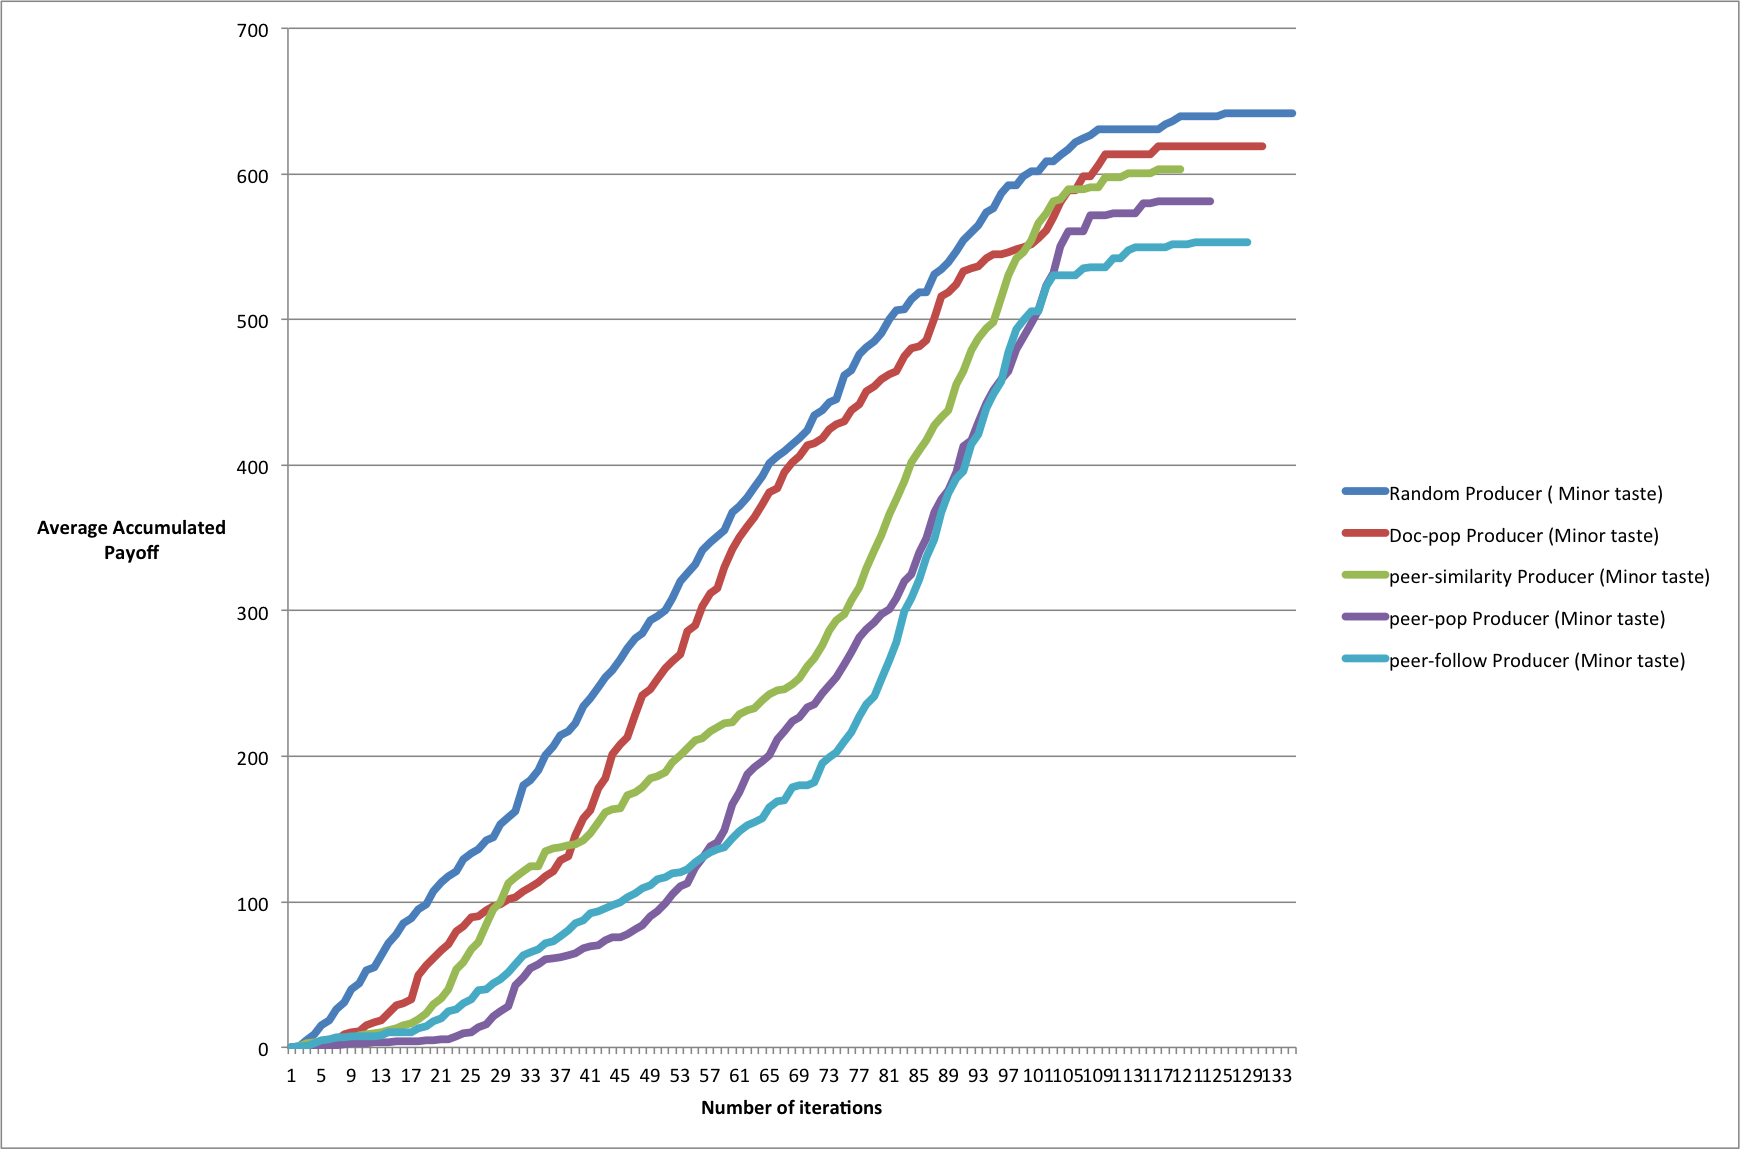
\includegraphics[width=0.6\textwidth,center]{images/EXP8-Strategies_Prod-Minor-taste}
\caption{Producers with minor taste}
\label{fig:images/F12}
\end{center}
\end{figure}

In Figure \ref{fig:images/F13}, the performance of consumers with major taste shows the average accumulated payoff in $ peer-like-similarity > document-popularity > Random $.  


\begin{figure}[h!]
\begin{center}
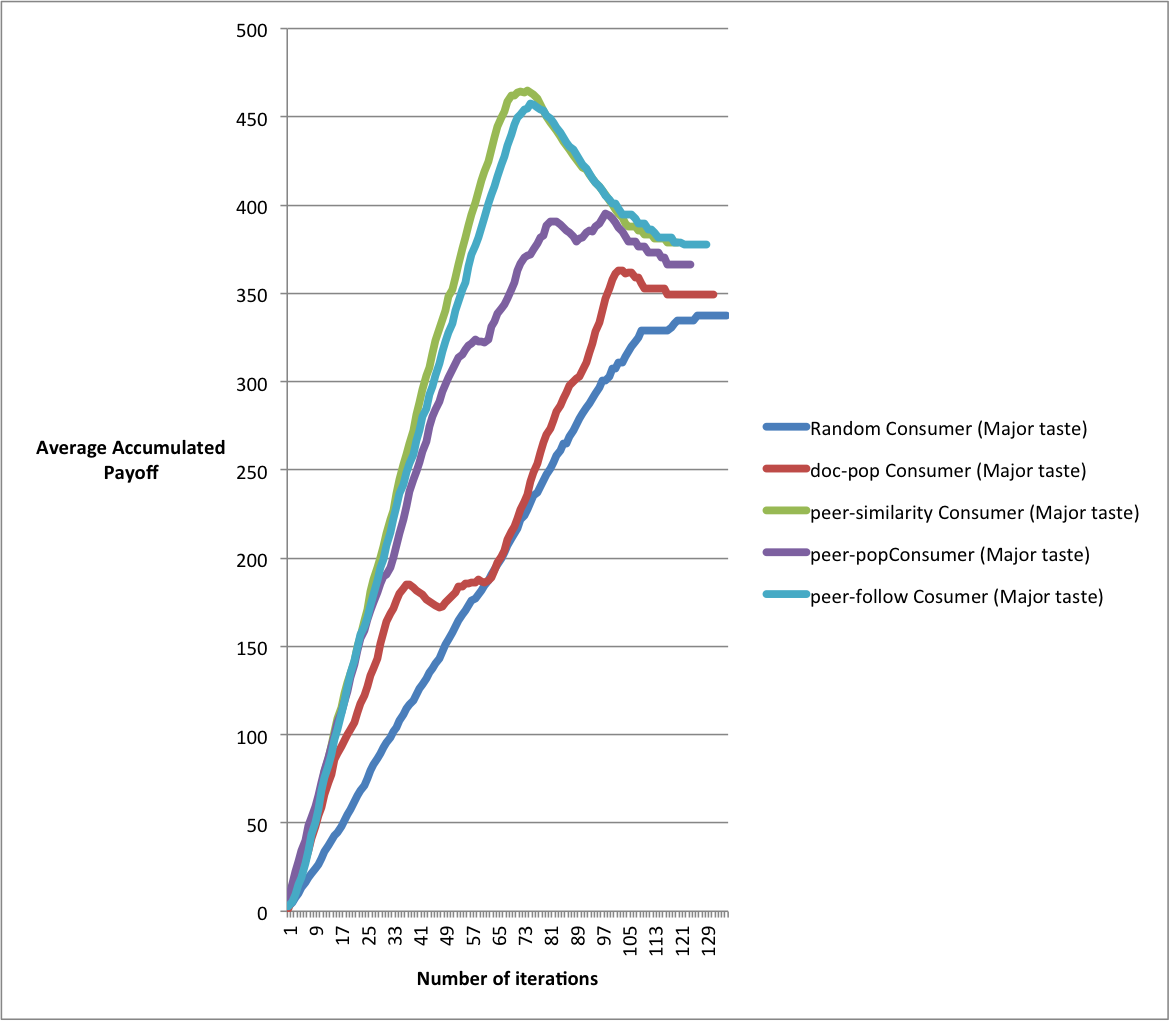
\includegraphics[width=0.6\textwidth,center]{images/EXP8-Strategies-cons-Major-taste.png}
\caption{Consumers with major taste}
\label{fig:images/F13}
\end{center}
\end{figure}


In Figure \ref{fig:images/F14} ,the performance of consumers with minor taste shows the average accumulated payoff in $ peer-like-similarity > Random > Document-popularity $.  


\begin{figure}[h!]
\begin{center}
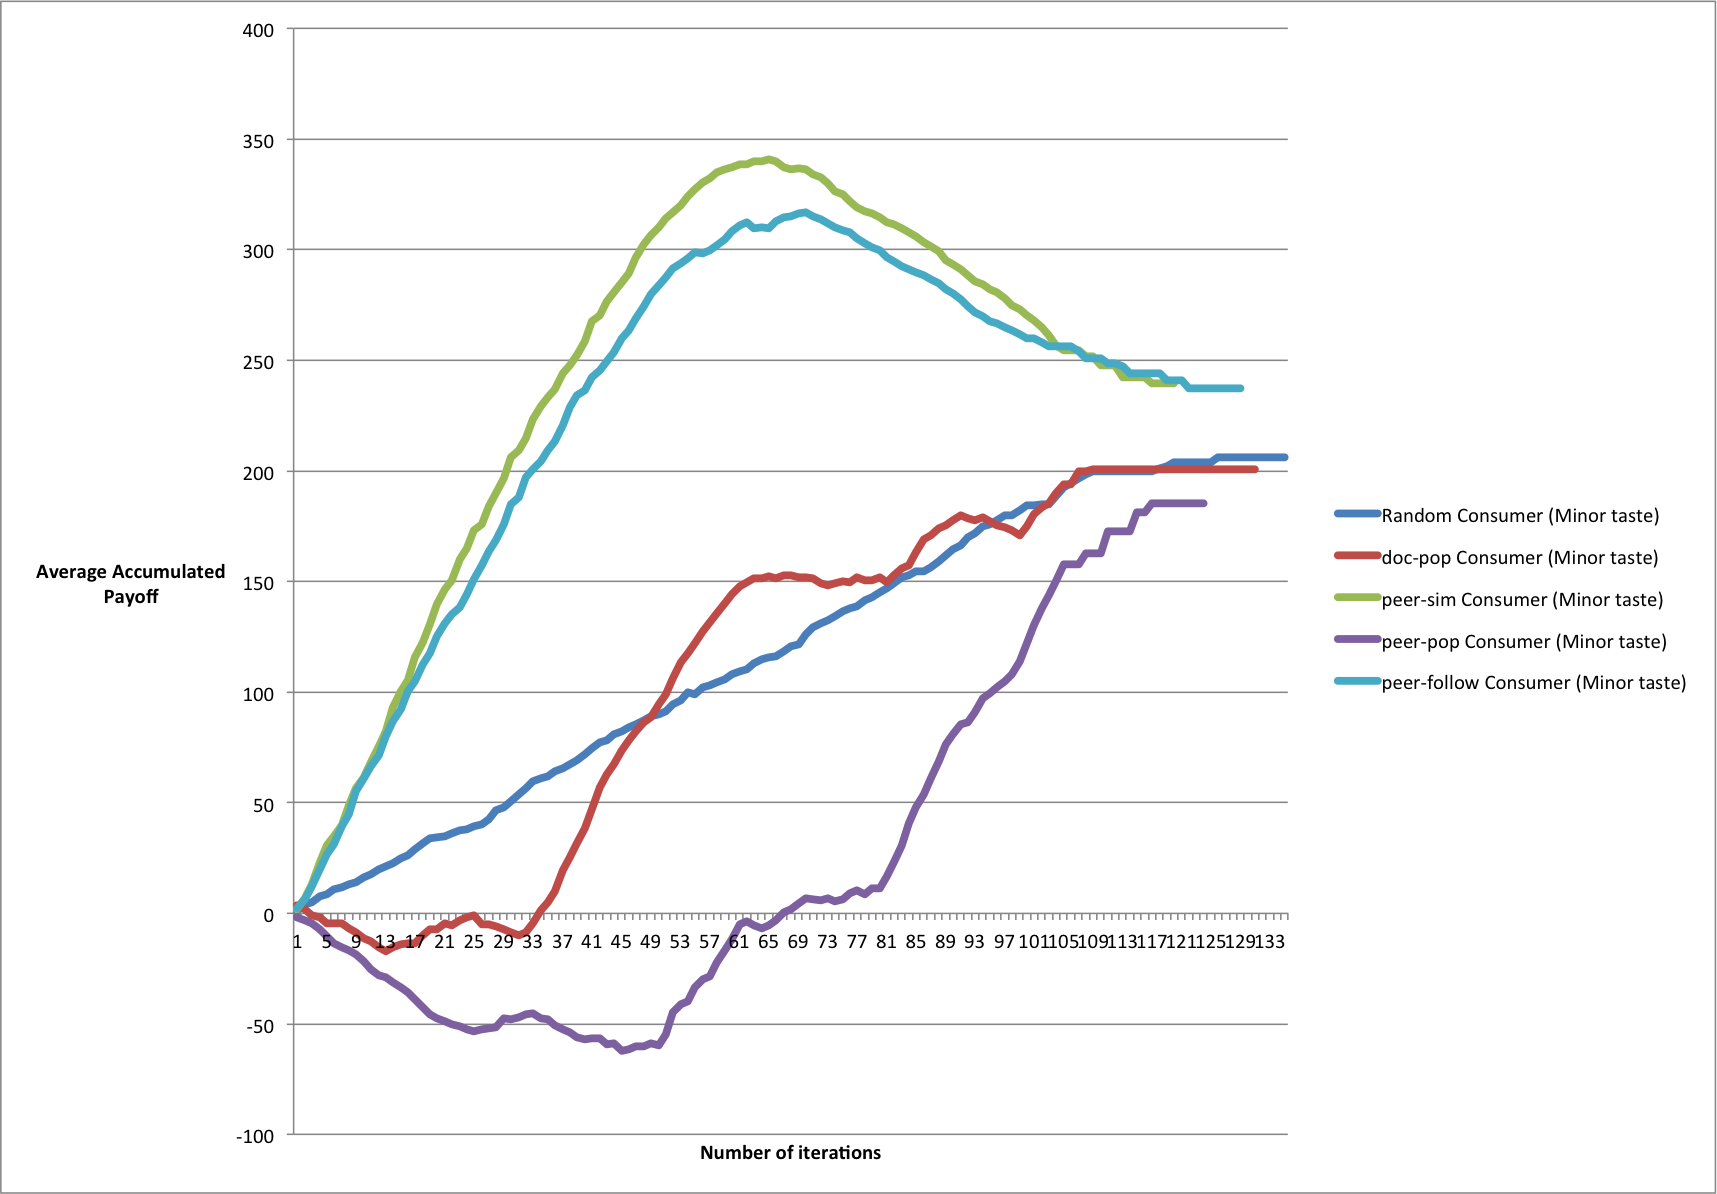
\includegraphics[width=0.6\textwidth,center]{images/EXP8-Strategies-cons-Minor-taste}
\caption{Consumers with minor taste}
\label{fig:images/F14}
\end{center}
\end{figure}


\subsection{Experiment 9}
\subsubsection{Goal}
 Study the relationship of average accumulated payoff with the number of iterations  
in document-popularity strategies for different ratio of major-minor consumers ( 90-10 and 70-30)

\subsubsection{Hypothesis}

As we saw in the result of experiment 4, document popularity strategy performance is proportional to  the number of peers with common taste.
As a result, when the number of peers with major taste increases, from 70\% to 90\% we expect higher amount of payoff for the peers with major taste.
and when the number of peers with minor taste decreases from 30\% to 10\% we would expect lower amount of payoff for the peers with minor taste.   


\subsubsection{Experiment Settings}

The simulation metrics and their values within the experiment are as the following.

\begin{table}[h!]
\caption{Document filtering strategies}
\begin{center}


\begin{tabular}{|c|c|}
\hline
K   & 5 \\ \hline
\# of iterations & 80 \\ \hline
\end{tabular}


\end{center}
\label{default}
\end{table}


\begin{table}[h!]
\caption{setting 1}
\begin{center}


\begin{tabular}{|c|c|}
\hline

Total \# of Documents &  400  \\ \hline
\# of Documents with tag 0 &  200  \\ \hline
\# of Documents with tag 1 &  200  \\ \hline

Total \# of peers & 60 \\ \hline

\# of consumer peers with taste 1  & 54 \\ \hline 
\# of consumer peers with taste 0  &  6\\ \hline

Ranking strategies of consumer peers with taste 1  & document-popularity \\ \hline 
Ranking strategies of consumer peers with taste 0  &  document-popularity\\ \hline


\end{tabular}

\end{center}
\label{default}
\end{table}



\begin{table}[h!]
\caption{setting 2}
\begin{center}


\begin{tabular}{|c|c|}
\hline

Total \# of Documents &  400  \\ \hline
\# of Documents with tag 0 &  200  \\ \hline
\# of Documents with tag 1 &  200  \\ \hline

Total \# of peers & 60 \\ \hline
\# of consumer peers with taste 1  &  48 \\ \hline 
\# of consumer peers with taste 0  &  12 \\ \hline

Ranking strategies of consumer peers with taste 1  & document-popularity \\ \hline 
Ranking strategies of consumer peers with taste 0  &  document-popularity\\ \hline

\end{tabular}

\end{center}
\label{default}
\end{table}



\begin{table}[h!]
\caption{Document tags and peer's tastes}

\begin{center}

\begin{tabular}{|c|c|}
\hline tag/taste values & (0 1 )\\
\hline \# of document tags   &  1\\ \hline 
\# of peer tastes  &  1 \\ \hline 
\end{tabular}

\end{center}
\label{default}
\end{table}


\subsubsection{Results and Discussion}

\begin{figure}[h!]
\begin{center}
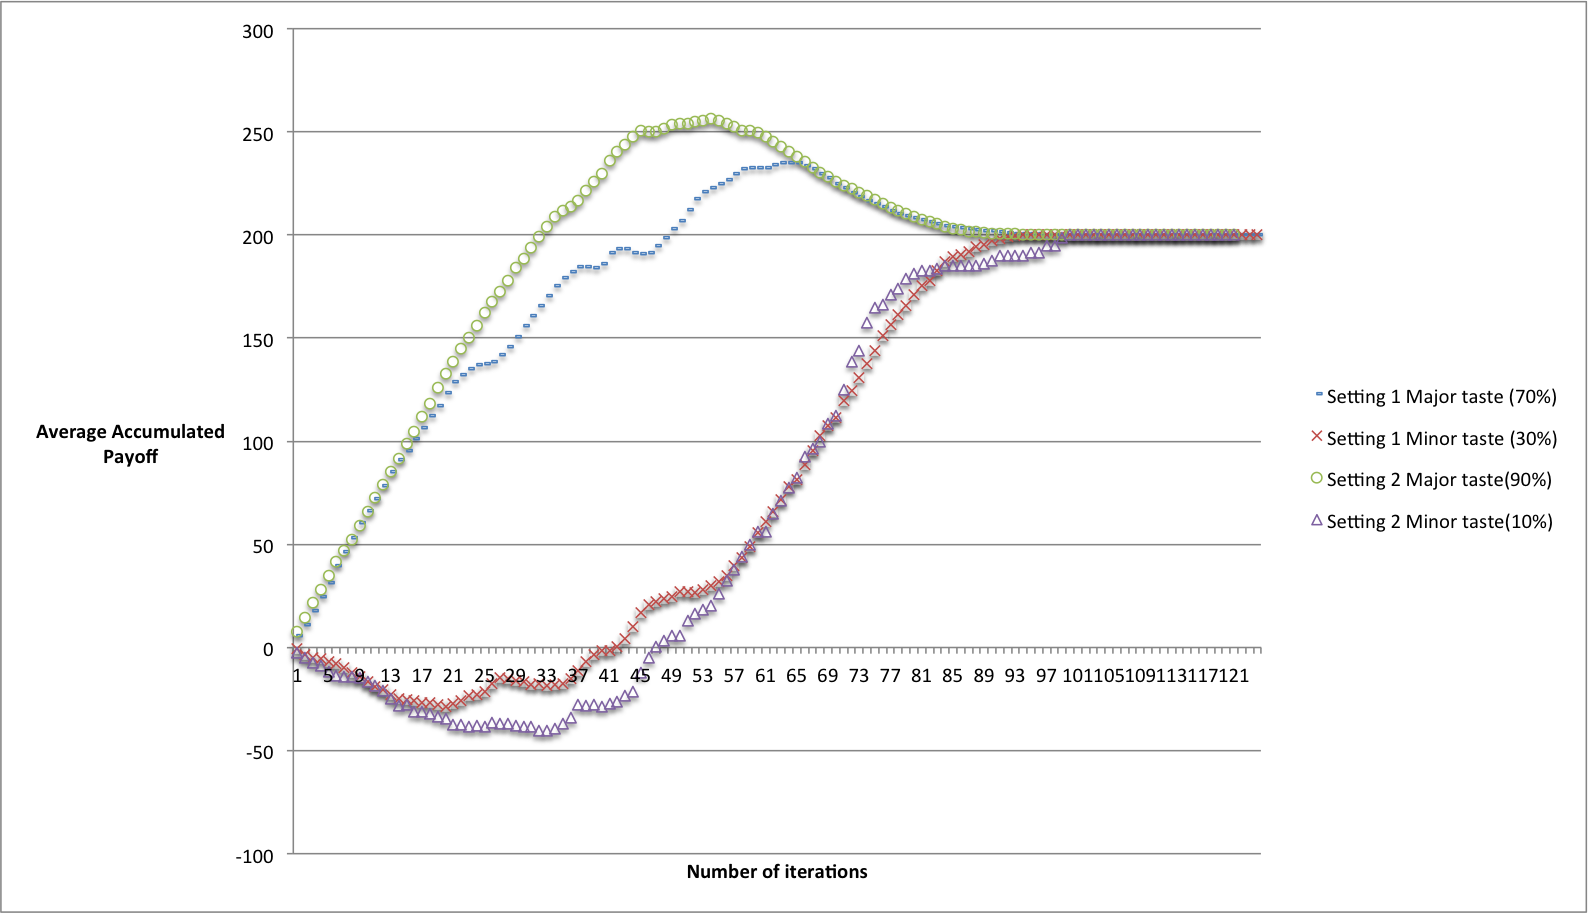
\includegraphics[width=0.8\textwidth,center]{images/EXP9-doc-pop-twoSettings-MajorMinor}
\caption{The average accumulated payoff in document-popularity for settings with different ratios of major and minor consumers}
\end{center}
\end{figure}

As it was expected, the peers with majors tastes had a dramatically higher payoff in compared with the peers with minor tastes.
And increase the ratio of number of peers with major taste, increased their payoff, and decreased the payoff of peers with minor taste. 


\subsection{Experiment 10}
\subsubsection{Goal}

 Study the relationship of average accumulated payoff with the number of iterations  
in peer-like-similarity strategies for different ratio of major-minor consumers ( 90-10 and 70-30)

\subsubsection{Hypothesis}

As we saw in the result of Experiment 5, in peer-like-similarity strategy when the distribution of tastes among peers is uniform, 
or when there are peers with major and minor tastes, the  average accumulated payoff resulted in values close to the best strategy.
However, the peers with major tastes had a more steep slope of increase in compared with peers with minor tastes. 
We can predict that when the number of peers with minor tastes decreases, it would take a longer time for peers to visit the documents in the 
document space and therefore the number of common likes between peers grows slowly.  

\subsubsection{Experiment Settings}

The simulation metrics and their values within the experiment are as the following.

\begin{table}[h!]
\caption{Document filtering strategies}
\begin{center}


\begin{tabular}{|c|c|}
\hline
K   & 5 \\ \hline
\# of iterations & 80 \\ \hline
\end{tabular}


\end{center}
\label{default}
\end{table}


\begin{table}[h!]
\caption{setting 1}
\begin{center}


\begin{tabular}{|c|c|}
\hline

Total \# of Documents &  400  \\ \hline
\# of Documents with tag 0 &  200  \\ \hline
\# of Documents with tag 1 &  200  \\ \hline

Total \# of peers & 60 \\ \hline

\# of consumer peers with taste 1  & 54 \\ \hline 
\# of consumer peers with taste 0  &  6\\ \hline

Ranking strategies of consumer peers with taste 1  & peer-like-similarity \\ \hline 
Ranking strategies of consumer peers with taste 0  &  peer-like-similarity\\ \hline


\end{tabular}

\end{center}
\label{default}
\end{table}



\begin{table}[h!]
\caption{setting 2}
\begin{center}


\begin{tabular}{|c|c|}
\hline

Total \# of Documents &  400  \\ \hline
\# of Documents with tag 0 &  200  \\ \hline
\# of Documents with tag 1 &  200  \\ \hline

Total \# of peers & 60 \\ \hline
\# of consumer peers with taste 1  &  48 \\ \hline 
\# of consumer peers with taste 0  &  12 \\ \hline

Ranking strategies of consumer peers with taste 1  & peer-like-similarity \\ \hline 
Ranking strategies of consumer peers with taste 0  &  peer-like-similarity\\ \hline

\end{tabular}

\end{center}
\label{default}
\end{table}



\begin{table}[h!]
\caption{Document tags and peer's tastes}

\begin{center}

\begin{tabular}{|c|c|}
\hline tag/taste values & (0 1 )\\
\hline \# of document tags   &  1\\ \hline 
\# of peer tastes  &  1 \\ \hline 
\end{tabular}

\end{center}
\label{default}
\end{table}


\subsubsection{Results and Discussion}



\begin{figure}[h!]
\begin{center}
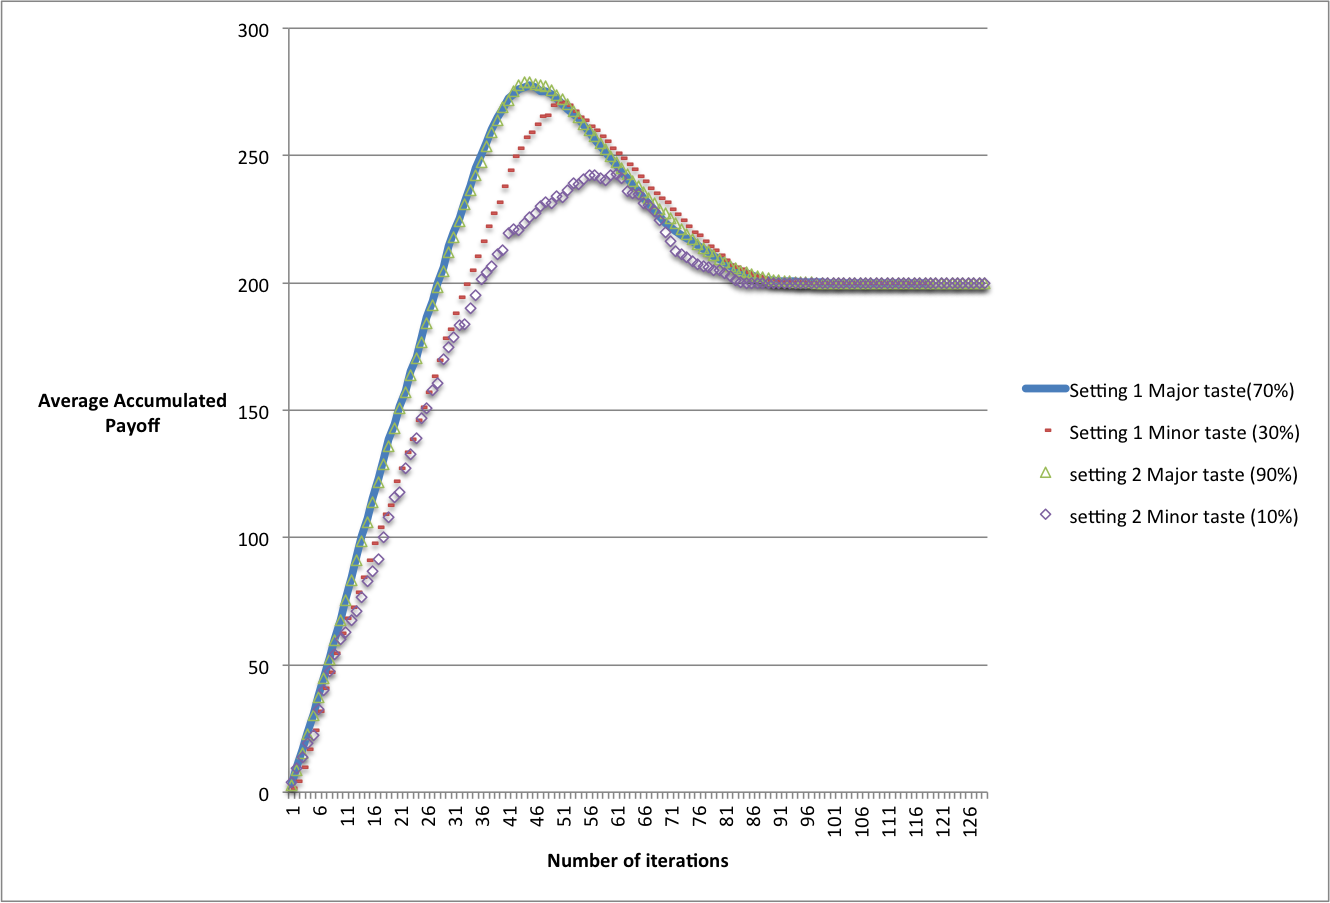
\includegraphics[width=0.8\textwidth,center]{images/EXP10-peer-sim-twoSettings-MajorMinor}
\caption{The average accumulated payoff in peer-like-similarity for settings with different ratios of major and minor consumers}
\end{center}
\end{figure}


The result of experiment showed what we expected from our hypotheses. The slope of average accumulated payoff got lower when the number of 
peers with similar taste were decreased.  


\subsection{Experiment 11}
\subsubsection{Goal}
 Study the relationship of average accumulated payoff with the number of iterations  
 when some consumers use document-popularity strategy and the rest of consumers use peer-similarity 
strategy, with two different settings: 1. Major taste consumers use document-popularity strategy. 2. Major taste consumers
use peer-like-similarity strategy.


\subsubsection{Hypothesis}

This experiment studies the effect of document-popularity and peer-like-similarity strategies on each other, 
when each strategy is used by major or minor taste consumers following the the two settings below:

Setting1, when Major taste consumers use document-popularity and minor taste consumers use peer-like-similarity:
 
We expect that minor taste consumers that use peer-similarity strategy would affect the performance of major taste consumers that use document popularity strategy.  
Since peer-like-similarity strategy has a performance close to the best strategy even for the minor taste consumers, it would cause minor taste consumers
to like more documents, and therefore increase the numer of likes of the documents with minor taste. As a result, 
document-popularity would use those  minor taste documents in its topK, which would make its consumers payoff to drop dramatically. 

Setting2, when Major taste consumers use peer-like-similarity and minor taste consumers use document-popularity:

This case is similar to the hypothesis for setting 1, with this difference that the  consumers payoff that use document popularity would be lower than
the one in setting 1.  


\subsubsection{Experiment Settings}

The simulation metrics and their values within the experiment are as the following.

\begin{table}[h!]
\caption{Document filtering strategies}
\begin{center}


\begin{tabular}{|c|c|}
\hline
K   & 5 \\ \hline
\# of iterations & 80 \\ \hline
\end{tabular}


\end{center}
\label{default}
\end{table}


\begin{table}[h!]
\caption{setting 1}
\begin{center}


\begin{tabular}{|c|c|}
\hline

Total \# of Documents &  400  \\ \hline
\# of Documents with tag 0 &  200  \\ \hline
\# of Documents with tag 1 &  200  \\ \hline

Total \# of peers & 60 \\ \hline

\# of consumer peers with taste 1  & 48 \\ \hline 
\# of consumer peers with taste 0  &  12\\ \hline

Ranking strategies of consumer peers with taste 1  & document-popularity \\ \hline 
Ranking strategies of consumer peers with taste 0  &  peer-like-similarity\\ \hline


\end{tabular}

\end{center}
\label{default}
\end{table}



\begin{table}[h!]
\caption{setting 2}
\begin{center}


\begin{tabular}{|c|c|}
\hline

Total \# of Documents &  400  \\ \hline
\# of Documents with tag 0 &  200  \\ \hline
\# of Documents with tag 1 &  200  \\ \hline

Total \# of peers & 60 \\ \hline
\# of consumer peers with taste 1  &  48 \\ \hline 
\# of consumer peers with taste 0  &  12 \\ \hline

Ranking strategies of consumer peers with taste 1  & peer-like-similarity \\ \hline 
Ranking strategies of consumer peers with taste 0  &  document-popularity\\ \hline

\end{tabular}

\end{center}
\label{default}
\end{table}



\begin{table}[h!]
\caption{Document tags and peer's tastes}

\begin{center}

\begin{tabular}{|c|c|}
\hline tag/taste values & (0 1 )\\
\hline \# of document tags   &  1\\ \hline 
\# of peer tastes  &  1 \\ \hline 
\end{tabular}

\end{center}
\label{default}
\end{table}



\subsubsection{Results and Discussion}

The result indicated the negative effect of peer-like-similarity strategy of a group peers,
on the rest of peers who use document-popularity strategy. The negative effect was worse in
setting 2 of experiment were the minor taste consumers were using document-popularity strategy. 


\begin{figure}[h!]
\begin{center}
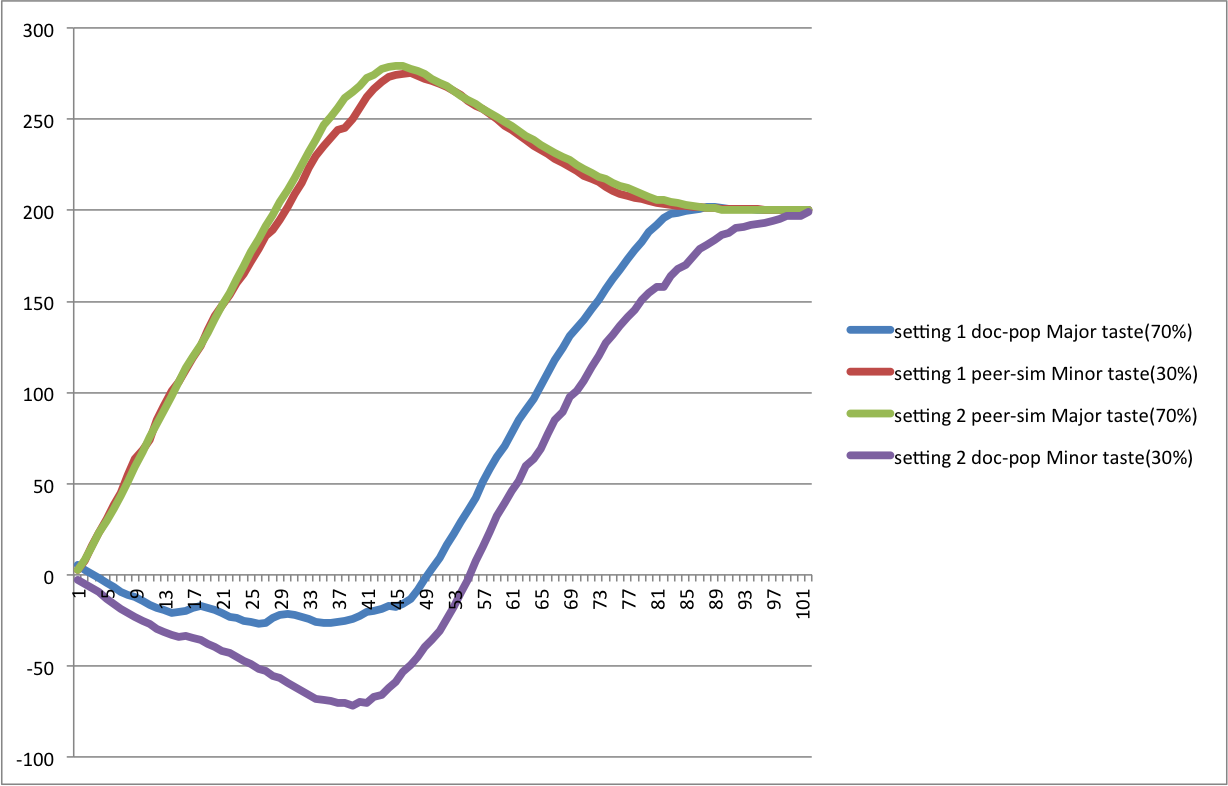
\includegraphics[width=0.8\textwidth,center]{images/EXP11-doc-pop-peer-sim-MajorMinor}
\caption{The average accumulated payoff when major taste consumers use document-popularity and the rest of consumers use peer-like-similarity}
\end{center}
\end{figure}

\subsection{Experiment 12}
\subsubsection{Goal}

 Study the relationship of average accumulated payoff with the number of iterations  
in peer-popularity strategies for different ratio of major-minor consumers ( 90-10 and 70-30)

\subsubsection{Hypothesis}
The peer-popularity of a peer increases, when the number of its followers increases, 
this is the case, when the peers like a documents that is already liked by peer. 

Therefore, once a peer likes a document, every other peers of the same taste that visit and liked that document, would end up
following that peer. Therefore, the peer-popularity of a peer increases more when the number of common documents likes between the 
two peers increases. As a result, we should expect a performance similar to peer-like-similarity strategy for the two settings. 



\subsubsection{Experiment Settings}

The simulation metrics and their values within the experiment are as the following.

\begin{table}[h!]
\caption{Document filtering strategies}
\begin{center}


\begin{tabular}{|c|c|}
\hline
K   & 5 \\ \hline
\# of iterations & 80 \\ \hline
\end{tabular}


\end{center}
\label{default}
\end{table}


\begin{table}[h!]
\caption{setting 1 of agents populations}
\begin{center}


\begin{tabular}{|c|c|}
\hline

Total \# of Documents &  400  \\ \hline
\# of Documents with tag 0 &  200  \\ \hline
\# of Documents with tag 1 &  200  \\ \hline

Total \# of peers & 60 \\ \hline

\# of consumer peers with taste 1  & 54 \\ \hline 
\# of consumer peers with taste 0  &  6\\ \hline

Ranking strategies of consumer peers with taste 1  & peer-popularity \\ \hline 
Ranking strategies of consumer peers with taste 0  &  peer-popularity\\ \hline


\end{tabular}

\end{center}
\label{default}
\end{table}



\begin{table}[h!]
\caption{setting 2 of agents populations}
\begin{center}


\begin{tabular}{|c|c|}
\hline

Total \# of Documents &  400  \\ \hline
\# of Documents with tag 0 &  200  \\ \hline
\# of Documents with tag 1 &  200  \\ \hline

Total \# of peers & 60 \\ \hline
\# of consumer peers with taste 1  &  48 \\ \hline 
\# of consumer peers with taste 0  &  12 \\ \hline

Ranking strategies of consumer peers with taste 1  & peer-popularity \\ \hline 
Ranking strategies of consumer peers with taste 0  &  peer-popularity\\ \hline

\end{tabular}

\end{center}
\label{default}
\end{table}



\begin{table}[h!]
\caption{Document tags and peer's tastes}

\begin{center}

\begin{tabular}{|c|c|}
\hline tag/taste values & (0 1 )\\
\hline \# of document tags   &  1\\ \hline 
\# of peer tastes  &  1 \\ \hline 
\end{tabular}

\end{center}
\label{default}
\end{table}


\subsubsection{Results and Discussion}

As the result shows, the payoff drops dramatically for minor consumers and gets worse the difference between 
the number of major and minor consumers becomes larger. We can conclude that similar to document-strategy,
in peer-popularity strategy, the peer-popularity metric is calculated similarly for all the minor and major consumers.
This would result, in benefitting major consumers with a performance close to performance in peer-like-similarly and
and would lower the payoff of minor consumers dramatically.  

\begin{figure}[h!]
\begin{center}
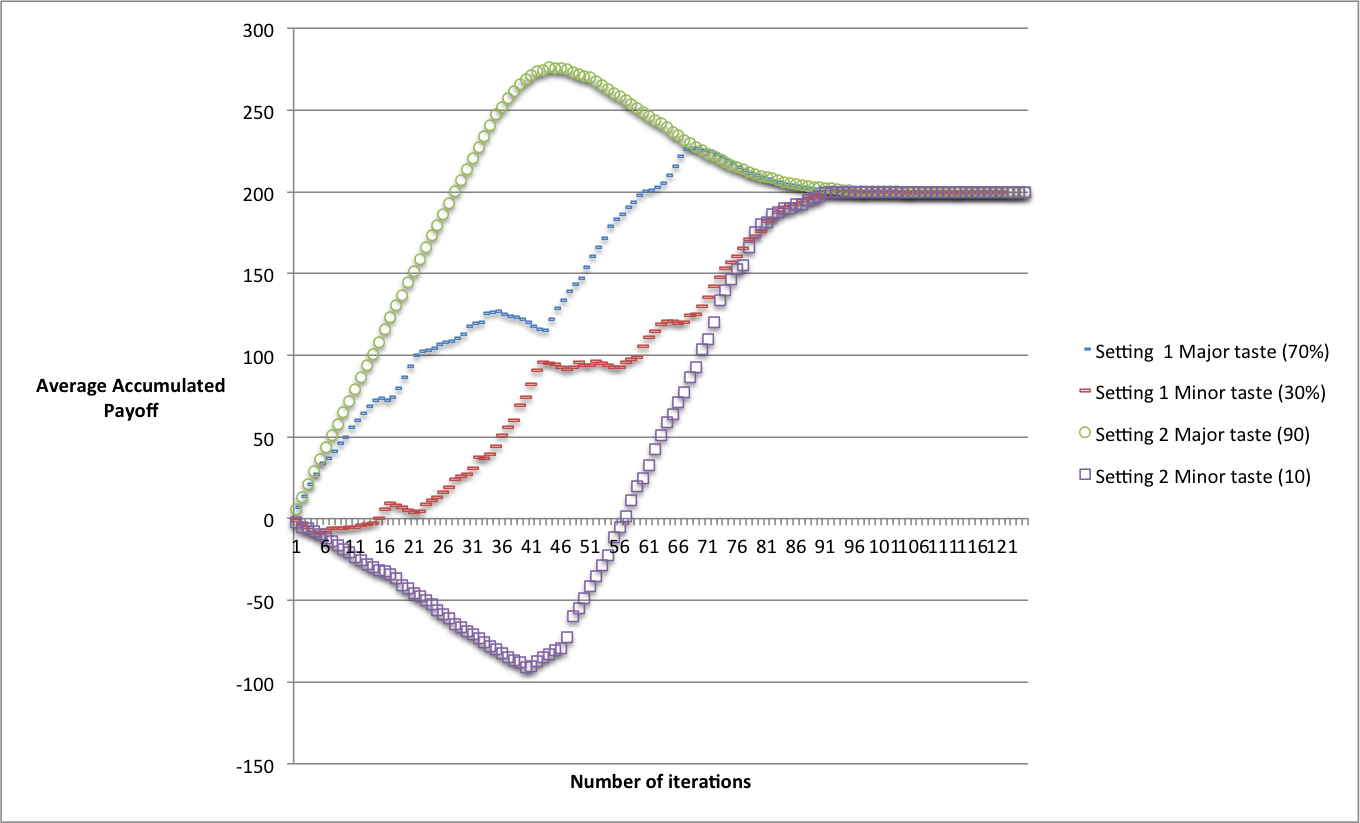
\includegraphics[width=0.8\textwidth,center]{images/EXP12-peer-pop-twoSettings-MajorMinor}
\caption{The average accumulated payoff in peer-popularity and peer-similarity strategies}
\end{center}
\end{figure}


\subsection{Experiment 13}
\subsubsection{Goal}
Study the effect of peer-popularity and peer-like-similarity strategies on each other, 
when each strategy is used by major or minor taste consumers following the the two settings below:
 1. Major taste consumers use peer-popularity strategy. 2. Major taste consumers
use peer-like-similarity strategy.

\subsubsection{Hypothesis}


In Setting1, when Major taste consumers use peer-popularity and minor taste consumers use peer-like-similarity:
 
We expect that major taste consumers that use peer-popularity strategy would perform similar to major taste consumers that use peer-like-similarity strategy. And since the performance of 
major and minor consumers in peer-like-similarity are close to each other, therefore, the consumers of the two strategies would have the slop of their payoff changes very close to each other.  

Setting2, when Major taste consumers use peer-like-similarity and minor taste consumers use peer-popularity:

This case is similar to the hypothesis for setting 1, with this difference that minor taste consumers would benefit less from peer-popularity strategy and therefore major taste consumers
that use peer-like-similarity strategy would have a better payoff


\subsubsection{Experiment Settings}

The simulation metrics and their values within the experiment are as the following.

\begin{table}[h!]
\caption{Document filtering strategies}
\begin{center}


\begin{tabular}{|c|c|}
\hline
K   & 5 \\ \hline
\# of iterations & 80 \\ \hline
\end{tabular}


\end{center}
\label{default}
\end{table}


\begin{table}[h!]
\caption{setting 1}
\begin{center}


\begin{tabular}{|c|c|}
\hline

Total \# of Documents &  400  \\ \hline
\# of Documents with tag 0 &  200  \\ \hline
\# of Documents with tag 1 &  200  \\ \hline

Total \# of peers & 60 \\ \hline

\# of consumer peers with taste 1  & 48 \\ \hline 
\# of consumer peers with taste 0  &  12\\ \hline

Ranking strategies of consumer peers with taste 1  & peer-popularity \\ \hline 
Ranking strategies of consumer peers with taste 0  &  peer-like-similarity\\ \hline


\end{tabular}

\end{center}
\label{default}
\end{table}



\begin{table}[h!]
\caption{setting 2}
\begin{center}


\begin{tabular}{|c|c|}
\hline

Total \# of Documents &  400  \\ \hline
\# of Documents with tag 0 &  200  \\ \hline
\# of Documents with tag 1 &  200  \\ \hline

Total \# of peers & 60 \\ \hline
\# of consumer peers with taste 1  &  48 \\ \hline 
\# of consumer peers with taste 0  &  12 \\ \hline

Ranking strategies of consumer peers with taste 1  & peer-like-similarity \\ \hline 
Ranking strategies of consumer peers with taste 0  &  peer-popularity\\ \hline

\end{tabular}

\end{center}
\label{default}
\end{table}



\begin{table}[h!]
\caption{Document tags and peer's tastes}

\begin{center}

\begin{tabular}{|c|c|}
\hline tag/taste values & (0 1 )\\
\hline \# of document tags   &  1\\ \hline 
\# of peer tastes  &  1 \\ \hline 
\end{tabular}

\end{center}
\label{default}
\end{table}


\subsubsection{Results and Discussion}

The result of the experiment showed that major consumers that use peer-popularity have a performance similar to the performance of major consumers in peer-like-similarity, 
and minor consumers that used peer-popularity had a similar performance to minor consumers that used peer-like-similarity.

The result of this expriment, indicate that the peer-popularity and peer-like-similarity strategies do not have a significant negative effect on the performance of each other. 


\begin{figure}[h!]
\begin{center}
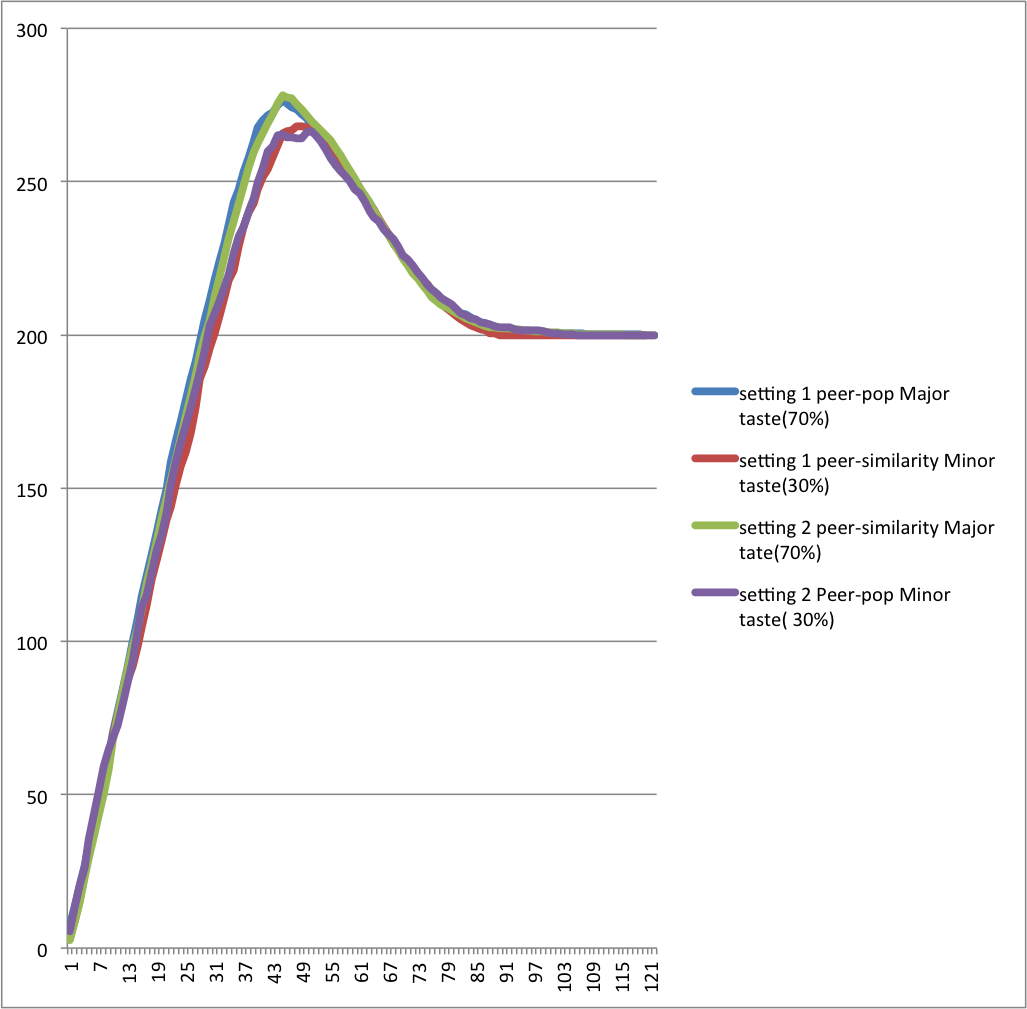
\includegraphics[width=0.8\textwidth,center]{images/EXP13-peer-pop-peer-sim-MajorMinor}
\caption{The average accumulated payoff when major taste consumers use peer-popularity and the rest of consumers use peer-like-similarity}
\end{center}
\end{figure}


\section{Conclusion}
[TO DO]
%\nocite{*}
\bibliographystyle{unsrt} \bibliography{refs} 	  
\end{document}